%%%%%%%%%%%%%%%%%%%%%%%%%%%%%%%%%%%%%%%%%%%%%%%%%%%
%
%  New template code for TAMU Theses and Dissertations starting Fall 2012.  
%  For more info about this template or the 
%  TAMU LaTeX User's Group, see http://www.howdy.me/.
%
%  Author: Wendy Lynn Turner 
%
%%%%%%%%%%%%%%%%%%%%%%%%%%%%%%%%%%%%%%%%%%%%%%%%%%%

\documentclass[12pt]{report}
\usepackage[letterpaper]{geometry}
\geometry{verbose,tmargin=1.25in,bmargin=1.25in,lmargin=1.4in,rmargin=1.15in}
 \usepackage[doublespacing]{setspace}
 \usepackage{tocloft}
 \usepackage[rm, tiny,center, compact]{titlesec}
 \usepackage{indentfirst}
 \usepackage{etoolbox}
\usepackage{tocvsec2}
 \usepackage[titletoc]{appendix}
 \usepackage{appendix}
% \usepackage{tamuconfig}
 \usepackage{pvamuconfig}
\usepackage{rotating}

%\usepackage{fancyhdr}
%\fancypagestyle{plain}{%
%\renewcommand{\headrulewidth}{0pt}%
%\fancyhf{}%
%\rhead{\thepage}%
%}

% Change the default page style to upper-righter page number
\usepackage{etoolbox}% http://ctan.org/pkg/etoolbox
\patchcmd{\chapter}% <cmd>
  {plain}% <search>
  {myheadings}% <replace>
  {}{}% <success><failure>

% Added to fix issues with pdf searching in some versions of LaTeX
%\usepackage[T1]{fontenc}\usepackage{lmodern}
%%%%%%%%%%%%%%%%%%%%%%%%%%%%%
\usepackage{float}
\usepackage{listings}
\usepackage{color}
\definecolor{gray}{rgb}{0.4,0.4,0.4}
\definecolor{darkblue}{rgb}{0.0,0.0,0.6}
\definecolor{cyan}{rgb}{0.0,0.6,0.6}

\lstset{
  basicstyle=\ttfamily,
  columns=fullflexible,
  showstringspaces=false,
  commentstyle=\color{gray}\upshape
}

\lstdefinelanguage{XML}
{
  morestring=[b]",
  morestring=[s]{>}{<},
  morecomment=[s]{<?}{?>},
  stringstyle=\color{black},
  identifierstyle=\color{darkblue},
  keywordstyle=\color{cyan},
  morekeywords={xmlns,version,type}% list your attributes here
}

\usepackage{pbox}

%\usepackage{caption}
\usepackage[labelsep=period]{caption}
\usepackage{subcaption}
\usepackage{breakcites}
\usepackage{url}
\usepackage{tabularx}

\usepackage{array}
\newcolumntype{L}[1]{>{\raggedright\let\newline\\\arraybackslash\hspace{0pt}}m{#1}}
\newcolumntype{C}[1]{>{\centering\let\newline\\\arraybackslash\hspace{0pt}}m{#1}}
\newcolumntype{R}[1]{>{\raggedleft\let\newline\\\arraybackslash\hspace{0pt}}m{#1}}

\usepackage{textcomp}
\usepackage{adjustbox}
\usepackage{blindtext}

% Hyperref setup below.  You should be able to get away with using uncommenting just the first line.
%\usepackage[hidelinks]{hyperref}

% if \usepackage[hidelinks]{hyperref} doesn't work try this.
% \usepackage{hyperref}  % Hidelinks is an option that removes link visiability.  TAMU Thesis Offices prefers to not see the links. But often doesn't work.  
% 
% \hypersetup{
%     colorlinks=true,
%     linkcolor=black,
%     citecolor=black,
%     filecolor=black,
%     urlcolor=black,
% }
%%%%%%%  End of hyperref setup.  One of these two options should work, but my motto with hyperref is when in doubt, comment it out!
%%%%%%%%%  This hopefully fixes the problem with vertical spacing of section headings at the top of the page..  Commented out in 1.0.7
% \preto\section{%
% \ifnum\value{section}>0\addtocontents{toc}{\vskip-6pt}\fi
% }
% \preto\subsection{%
% \ifnum\value{subsection}=0\addtocontents{toc}{\vskip-6pt}\fi
% \ifnum\value{subsection}>0\addtocontents{toc}{\vskip-6pt}\fi
% } 
%%%%%%%%%%%%%%%%%%%%%%%%%%%%%%%%%%%%%%%%%%%%%%%%%%%%%%

\begin{document}

% Change to PVAMU format
\ifx true false 
\renewcommand{\tamumanuscripttitle}{A Scalable and Distributed Seismic Data Toolkit on Big Data Analytics Platform}
\renewcommand{\tamupapertype}{Dissertation}
\renewcommand{\tamufullname}{Chao Chen}
\renewcommand{\tamudegree}{Master Degree}
\renewcommand{\tamuchairone}{Dr. Lei Huang}
% Uncomment out the next line if you have co-chairs.  You will also need to edit the titlepage.tex file.
%\newcommand{\tamuchairtwo}{Additional Chair Name}
\renewcommand{\tamumemberone}{Dr. Lei Huang}
\newcommand{\tamumembertwo}{Dr. Lin Li}
\newcommand{\tamumemberthree}{Dr. Sherri S. Frizell}
\renewcommand{\tamudepthead}{Dr. Yonggao Yang}
\renewcommand{\tamugradmonth}{December}
\renewcommand{\tamugradyear}{2016}
\renewcommand{\tamudepartment}{Department of Computer Science}
\fi

\renewcommand{\pvamucollege}{PRAIRIE VIEW A\protect\&M UNIVERSITY\protect\\COLLEGE OF ENGINEERING\protect\\PRAIRIE VIEW, TEXAS}
\renewcommand{\pvamumanuscripttitle}{A Scalable and Distributed Seismic Data Toolkit on Big Data Analytics Platform}
\renewcommand{\pvamupapertype}{Thesis}
\renewcommand{\pvamusubmitto}{Submitted to the Graduate School\\In Partial Fulfillment of the Requirements for\\The Degree of}
\renewcommand{\pvamudegree}{MASTER OF SCIENCE}
\renewcommand{\pvamumajor}{COMPUTER SCIENCE}
\renewcommand{\pvamufullname}{Chao Chen}
\renewcommand{\pvamuadvisor}{Advisor Name}
\renewcommand{\pvamudepthead}{Department Head}
\renewcommand{\pvamucollegedean}{College Dean Name}
\renewcommand{\pvamugraddean}{Graduate School Dean Name}
\renewcommand{\pvamugradmonth}{December}
\renewcommand{\pvamugradyear}{2016}


%%%%%%%%%%%%%%%%%%%%%%%%%%%%%%%%%%%%%%%%%%%%%%%%%%%%
%
%  New template code for TAMU Theses and Dissertations starting Fall 2012.  
%  For more info about this template or the 
%  TAMU LaTeX User's Group, see http://www.howdy.me/.
%
%  Author: Wendy Lynn Turner 
%	 Version 1.0 
%  Last updated 8/5/2012
%
%%%%%%%%%%%%%%%%%%%%%%%%%%%%%%%%%%%%%%%%%%%%%%%%%%%

%%%%%%%%%%%%%%%%%%%%%%%%%%%%%% 
%% TITLE PAGE
%% The values get updated automatically.  Please do not make changes to this file other than adding/deleting committee members where necessary.
%%%%%%%%%%%%%%%%%%%%%%%%%%%%%%

\providecommand{\tabularnewline}{\\}



\begin{titlepage}
\begin{center}
\MakeUppercase{\tamumanuscripttitle}
\vspace{4em}

A \tamupapertype

by

\MakeUppercase{\tamufullname}

\vspace{4em}

\begin{singlespace}

Submitted to the Office of Graduate and Professional Studies of \\
Prairie View A\&M University \\

in partial fulfillment of the requirements for the degree of \\
\end{singlespace}

\MakeUppercase{\tamudegree}
\par\end{center}
\vspace{2em}
\begin{singlespace}
\begin{tabular}{ll}
 & \tabularnewline
& \cr
% If you have Co-Chairs comment out the 'Chair of Committee' line below and uncomment the 'Co-Chairs of Committee' line.
Chair of Committee, & \tamuchairone\tabularnewline
%Co-Chairs of Committee, & \tamuchairone\tabularnewline & \tamuchairtwo\tabularnewline
Committee Members, & \tamumemberone\tabularnewline
 & \tamumembertwo\tabularnewline
 & \tamumemberthree\tabularnewline
Head of Department, & \tamudepthead\tabularnewline

\end{tabular}
\end{singlespace}
\vspace{3em}

\begin{center}
\tamugradmonth \hspace{2pt} \tamugradyear

\vspace{3em}

Major Subject: \tamudepartment \par
\vspace{3em}
Copyright \tamugradyear \hspace{.5em}\tamufullname 
\par\end{center}
\end{titlepage}
\pagebreak{}




 % This is simply a file that formats and adds your titlepage, please do not edit this unless you have a specific need. .
%%%%%%%%%%%%%%%%%%%%%%%%%%%%%%%%%%%%%%%%%%%%%%%%%%%
%
%  New template code for TAMU Theses and Dissertations starting Fall 2012.  
%  For more info about this template or the 
%  TAMU LaTeX User's Group, see http://www.howdy.me/.
%
%  Author: Wendy Lynn Turner 
%	 Version 1.0 
%  Last updated 8/5/2012
%
%%%%%%%%%%%%%%%%%%%%%%%%%%%%%%%%%%%%%%%%%%%%%%%%%%%

%%%%%%%%%%%%%%%%%%%%%%%%%%%%%% 
%% TITLE PAGE
%% The values get updated automatically.  Please do not make changes to this file other than adding/deleting committee members where necessary.
%%%%%%%%%%%%%%%%%%%%%%%%%%%%%%

\providecommand{\tabularnewline}{\\}

\begin{titlepage}
\begin{center}

\begin{singlespace}
\MakeUppercase{\pvamucollege}
%PRAIRIE VIEW A\protect\&M UNIVERSITY\protect\\COLLEGE OF ENGINEERING\protect\\PRAIRIE VIEW, TEXAS\\

\vspace{10 mm}
\textbf{\MakeUppercase{\pvamumanuscripttitle}}

\vspace{5 mm}
A \pvamupapertype

\pvamusubmitto
%Submitted to the Graduate School\\In Partial Fulfillment of the Requirements for\\The Degree of\\

\vspace{5 mm}
\MakeUppercase{\pvamudegree}

IN

\MakeUppercase{\pvamumajor}

\vspace{10 mm}
\end{singlespace}

Submitted By:\\
\textbf{\MakeUppercase{\pvamufullname}}

\vspace{10 mm}
\par\end{center}

\begin{singlespace}
Certificate of Approval:

\vspace{10 mm}
\newcommand{\specialcell}[2][l]{%
  \begin{tabular}[#1]{@{}l@{}}#2\end{tabular}}

\begin{tabular}{L{7cm} L{7cm} }
       \specialcell{ \underline{\hspace{6cm}} \\ (Advisor\textquotesingle s name)\\Chairman\\Student Advisory Committee } 
            & \specialcell{ \underline{\hspace{6cm}} \\ (Department Head\textquotesingle s name)\\Department Head\\Computer Science Department }\\
       {} & {} \\
       {} & {} \\
       {} & {} \\
       \specialcell{ \underline{\hspace{6cm}} \\ (Dean\textquotesingle s name)\\Dean\\College of Engineering } 
            & \specialcell{ \underline{\hspace{6cm}} \\ (Graduate School Dean\textquotesingle s name)\\Acting Dean\\Graduate School }\\
\end{tabular}

\end{singlespace}

\vspace{3em}

\begin{center}
\pvamugradmonth \hspace{2pt} \pvamugradyear
\par\end{center}

\vspace{3em}

\end{titlepage}
\pagebreak{}





%%%%%%%%%%%%%%%%%%%%%%%%%%%%%%%%%%%%%%%%%%%%%%%%%%%
%
%  New template code for TAMU Theses and Dissertations starting Fall 2012.  
%  For more info about this template or the 
%  TAMU LaTeX User's Group, see http://www.howdy.me/.
%
%  Author: Wendy Lynn Turner 
%	 Version 1.0 
%  Last updated 8/5/2012
%
%%%%%%%%%%%%%%%%%%%%%%%%%%%%%%%%%%%%%%%%%%%%%%%%%%%

%%%%%%%%%%%%%%%%%%%%%%%%%%%%%% 
%% TITLE PAGE
%% The values get updated automatically.  Please do not make changes to this file other than adding/deleting committee members where necessary.
%%%%%%%%%%%%%%%%%%%%%%%%%%%%%%

\begin{titlepage}
\begin{center}

\vspace*{16 pt}
\MakeUppercase{\pvamumanuscripttitle}

\vspace{30 pt}
A \pvamupapertype

by

\MakeUppercase{\pvamufullname}

\vspace{30 pt}

\begin{singlespace}
Submitted to the Office of Graduate Studies of \\
Prairie View A\&M University \\
in partial fulfillment of the requirements for the degree of\\
\end{singlespace}

\vspace{16 pt}
\MakeUppercase{\pvamudegree}

\vspace{16 pt}

\end{center}

\begin{singlespace}
\hspace*{1ex} Approved as to style and content by:
\vspace{16 pt}
\newcommand{\specialcell}[2][l]{%
  \begin{tabular}[#1]{@{}l@{}}#2\end{tabular}}

\begin{tabular}{L{8cm} L{8cm} }
       \specialcell{ \underline{\hspace{6cm}} \\Lei Huang\\Chair of Committee } 
            & \specialcell{ \underline{\hspace{6cm}} \\Li Lin\\Committee Member }\\
       {} & {} \\
       \specialcell{ \underline{\hspace{6cm}} \\Sherri S. Frizell\\Committee Member } 
            & \specialcell{ \underline{\hspace{6cm}} \\Yonggao Yang\\Head of Department }\\
       {} & {} \\
       \specialcell{ \underline{\hspace{6cm}} \\Kendall T. Harris\\Dean, Roy G. Perry College of Engineering } 
            & \specialcell{ \underline{\hspace{6cm}} \\Cajetan M. Akujuobi\\Dean, Graduate Studies }\\
\end{tabular}

\end{singlespace}

\begin{center}
\vspace{22 pt}
\pvamugradmonth \hspace{2pt} \pvamugradyear \\
\vspace{22 pt}
Major Subject: Computer Science
\end{center}

\end{titlepage}
\pagebreak{}





%%%%%%%%%%%%%%%%%%%%%%%%%%%%%%%%%%%%%%%%%%%%%%%%%%%
%
%  New template code for TAMU Theses and Dissertations starting Fall 2012.  
%  For more info about this template or the 
%  TAMU LaTeX User's Group, see http://www.howdy.me/.
%
%  Author: Wendy Lynn Turner 
%	 Version 1.0 
%  Last updated 8/5/2012
%
%%%%%%%%%%%%%%%%%%%%%%%%%%%%%%%%%%%%%%%%%%%%%%%%%%%
%%%%%%%%%%%%%%%%%%%%%%%%%%%%%%%%%%%%%%%%%%%%%%%%%%%%%%%%%%%%%%%%%%%%%
%%                           ABSTRACT 
%%%%%%%%%%%%%%%%%%%%%%%%%%%%%%%%%%%%%%%%%%%%%%%%%%%%%%%%%%%%%%%%%%%%%

\chapter*{ABSTRACT}
\addcontentsline{toc}{chapter}{ABSTRACT} % Needs to be set to part, so the TOC doesnt add 'CHAPTER ' prefix in the TOC.

\pagestyle{plain} % No headers, just page numbers
\pagenumbering{roman} % Roman numerals
\setcounter{page}{2}

\begin{center}
\pvamumanuscripttitle

\pvamugradmonth \hspace{2pt} \pvamugradyear

\pvamufullname, B.S., southwest university of science and technology;

Chair of Advisory Committee: Dr. Lei Huang 

\par\end{center}

\indent Seismic volume is a basic data structure that has been widely used in geophysical computing, as well as in big data analytics applications of petroleum industry. It has been well studied in High Performance Computing (HPC) platforms. However, a little study has been done in big data analytics platforms. In this thesis, we present the work of designing and implementing an efficient Distributed Seismic Data Analytics Toolkit on top of Apache Spark big data analytics platform. The toolkit supports different ways of seismic volume data distributions, repartition, transposing, access, and data parallelism with a variety of parallel execution templates. This thesis also addresses the performance characteristics of these seismic volume data operations with different configurations, the services have been developed on top of this toolkit as well as the current status and future research plan of this big data analytics plaftorm. The scalability and parallelism are the main characteristics of this platform.  


 

\pagebreak{}

%%%%%%%%%%%%%%%%%%%%%%%%%%%%%%%%%%%%%%%%%%%%%%%%%%%%
%
%  New template code for TAMU Theses and Dissertations starting Fall 2012.  
%  For more info about this template or the 
%  TAMU LaTeX User's Group, see http://www.howdy.me/.
%
%  Author: Wendy Lynn Turner 
%	 Version 1.0 
%  Last updated 8/5/2012
%
%%%%%%%%%%%%%%%%%%%%%%%%%%%%%%%%%%%%%%%%%%%%%%%%%%%

%%%%%%%%%%%%%%%%%%%%%%%%%%%%%%%%%%%%%%%%%%%%%%%%%%%%%%%%%%%%%%%%%%%%%%
%%                           DEDICATION
%%%%%%%%%%%%%%%%%%%%%%%%%%%%%%%%%%%%%%%%%%%%%%%%%%%%%%%%%%%%%%%%%%%%%
\chapter*{DEDICATION}
\addcontentsline{toc}{chapter}{DEDICATION}  % Needs to be set to part, so the TOC doesnt add 'CHAPTER ' prefix in the TOC.



\indent This is an optional page.  Lorem ipsum dolor sit amet, consectetur adipiscing elit. Integer lectus quam, condimentum quis bibendum eu, sollicitudin eget lacus. Praesent non sodales odio. Class aptent taciti sociosqu ad litora torquent per conubia nostra, per inceptos himenaeos. Nulla ac luctus sapien. Morbi cursus sapien eget lorem fermentum hendrerit. Nam ac erat dui, in cursus velit. Vivamus hendrerit porttitor nisi, ut porttitor lorem volutpat eget. In ligula ligula, euismod ut condimentum sit amet, pulvinar sit amet diam. Pellentesque interdum, ipsum ullamcorper consequat dignissim, sem arcu egestas mauris, vitae interdum sem tortor ut ante. Nunc blandit laoreet nisi, non rutrum lorem hendrerit quis. Cras nunc diam, convallis et feugiat at, auctor id libero. Nunc facilisis massa eu eros imperdiet vestibulum. Vestibulum ante ipsum primis in faucibus orci luctus et ultrices posuere cubilia Curae; Donec non velit vitae tortor blandit semper.

Etiam vitae dolor nulla. Ut eros odio, rhoncus eget placerat vitae, elementum ac ante. Proin vitae odio eu nisl pharetra mattis. Pellentesque habitant morbi tristique senectus et netus et malesuada fames ac turpis egestas. Phasellus fermentum lacus consectetur neque consequat ullamcorper. Cras blandit urna non dui consequat molestie. Curabitur viverra nibh at nisi semper faucibus. Nam egestas mauris a enim dignissim nec consectetur tortor rutrum. Mauris at nisi in est luctus congue ut mattis est. Ut pretium, mi quis elementum cursus, ante eros suscipit ligula, ut porttitor elit leo sed turpis. Nam sed dui ligula.


\pagebreak{}

%%%%%%%%%%%%%%%%%%%%%%%%%%%%%%%%%%%%%%%%%%%%%%%%%%%
%
%  New template code for TAMU Theses and Dissertations starting Fall 2012.  
%  For more info about this template or the 
%  TAMU LaTeX User's Group, see http://www.howdy.me/.
%
%  Author: Wendy Lynn Turner 
%	 Version 1.0 
%  Last updated 8/5/2012
%
%%%%%%%%%%%%%%%%%%%%%%%%%%%%%%%%%%%%%%%%%%%%%%%%%%%


%%%%%%%%%%%%%%%%%%%%%%%%%%%%%%%%%%%%%%%%%%%%%%%%%%%%%%%%%%%%%%%%%%%%%%
%%                           ACKNOWLEDGEMENTS
%%%%%%%%%%%%%%%%%%%%%%%%%%%%%%%%%%%%%%%%%%%%%%%%%%%%%%%%%%%%%%%%%%%%%
\chapter*{ACKNOWLEDGEMENTS}
\addcontentsline{toc}{chapter}{ACKNOWLEDGEMENTS}  % Needs to be set to part, so the TOC doesnt add 'CHAPTER ' prefix in the TOC.

I would like to thank my advisor, professors, colleagues and friends who helped me a lot in the past two years. I cannot make it through and finish my thesis without your kind help.

First I want to thank my advisor Dr. Lei Huang, for giving me the chance to work in CloudComputing Lab, guiding my studies and researches in cloud computing. The facilities of CloudComputing Lab is a luxury for a student who want to do research on big data platforms. I would also like to thank Dr. Lin Li and Dr. Frizell, for spending lots of time to refine my thesis. Special thanks to Mr Ted Clee, for sharing his deep knowledge of seismic data analysis, which benefit me a lot in understanding so many geophysics terminologies in the use cases.

Also, I really appreciate all my colleagues and classmates worked in the lab in the past two years, for sharing so many interesting things from different cultures, and, of course, for helping and encouraging each other in work.

Finally I want to say thank you to my friend Yuzhong Yan, for always being the guy help me out at so many tough time in my life. I have learned so much from you not only as an engineer but also as a kind and wise man. Best wishes to you and your lovely family.

\pagebreak{}

\ifx true false
\vspace*{\fill}
\begin{center}
A.M.D.G.
\end{center}
\vspace*{\fill}
\pagebreak{}
\fi

%%%%%%%%%%%%%%%%%%%%%%%%%%%%%%%%%%%%%%%%%%%%%%%%%%%%
%
%  New template code for TAMU Theses and Dissertations starting Fall 2012.  
%  For more info about this template or the 
%  TAMU LaTeX User's Group, see http://www.howdy.me/.
%
%  Author: Wendy Lynn Turner 
%	 Version 1.0 
%  Last updated 8/5/2012
%
%%%%%%%%%%%%%%%%%%%%%%%%%%%%%%%%%%%%%%%%%%%%%%%%%%%

%%%%%%%%%%%%%%%%%%%%%%%%%%%%%%%%%%%%%%%%%%%%%%%%%%%%%%%%%%%%%%%%%%%%%%
%%                           NOMENCLATURE
%%%%%%%%%%%%%%%%%%%%%%%%%%%%%%%%%%%%%%%%%%%%%%%%%%%%%%%%%%%%%%%%%%%%%

\chapter*{NOMENCLATURE}
\addcontentsline{toc}{chapter}{NOMENCLATURE}  % Needs to be set to part, so the TOC doesnt add 'CHAPTER ' prefix in the TOC.

\begin{tabular}{ll}
B/CS  & Bryan/College Station\tabularnewline
HSUS & Humane Society of the United States\tabularnewline
P & Pressure\tabularnewline
T  & Time\tabularnewline
TVA & Tennessee Valley Authority\tabularnewline
TxDOT \hfill{}\hfill{}\hfill{}\hfill{}\hfill{}\hfill{}\hfill{}\hfill{} & \multicolumn{1}{l}{Texas Department of Transportation}\tabularnewline
\end{tabular}

\vspace{2em}

This page is optional.

\pagebreak{}

%%%%%%%%%%%%%%%%%%%%%%%%%%%%%%%%%%%%%%%%%%%%%%%%%%%
%
%  New template code for TAMU Theses and Dissertations starting Fall 2012.  
%  For more info about this template or the 
%  TAMU LaTeX User's Group, see http://www.howdy.me/.
%
%  Author: Wendy Lynn Turner 
%	 Version 1.7
%  Last updated 3/24/2014
%
%%%%%%%%%%%%%%%%%%%%%%%%%%%%%%%%%%%%%%%%%%%%%%%%%%%
%%%%%%%%%%%%%%%%%%%%%%%%%%%%%%%%%%%%%%%%%%%%%%%%%%%%%%%%%%%%%%%%%%%%%%
%%       TABLE OF CONTENTS
%%%%%%%%%%%%%%%%%%%%%%%%%%%%%%%%%%%%%%%%%%%%%%%%%%%%%%%%%%%%%%%%%%%%%
% single-space sections in Table of Contents  - commented in version 1.7
%\renewcommand{\cftsecafterpnum}{\vskip0.5\baselineskip}
%\renewcommand{\cftsubsecafterpnum}{\vskip0.5\baselineskip}
%\renewcommand{\cftsubsubsecafterpnum}{\vskip0.5\baselineskip}
%%%%%%%%%%%%%%%%%%%%%%%%%%%%%%%%%%%%%%%%%%%%%%%%%%%

\phantomsection
\addcontentsline{toc}{chapter}{TABLE OF CONTENTS}  

\begin{singlespace}
\renewcommand\contentsname{\normalfont} {\large\bfseries{\centerline{TABLE OF CONTENTS}}}

%\setcounter{tocdepth}{4} % This puts \subsubsection[]{×} in your List of Tables.  The default is 3.


%%%%%%%%%%%%%  Adds Page above the page number in TOC
\setlength{\cftaftertoctitleskip}{1em}
\renewcommand{\cftaftertoctitle}{%
\hfill{\normalfont {Page}\par}}



\tableofcontents

\end{singlespace}

\pagebreak{}

%%%%%%%%%%%%%%%%%%%%%%%%%%%%%%%%%%%%%%%%%%%%%%%%%%%%%%%%%%%%%%%%%%%%%%
%%                           LIST OF FIGURES
%%%%%%%%%%%%%%%%%%%%%%%%%%%%%%%%%%%%%%%%%%%%%%%%%%%%%%%%%%%%%%%%%%%%%

\phantomsection
\addcontentsline{toc}{chapter}{LIST OF FIGURES}  

%\renewcommand{\cftloftitlefont}{\large\bfseries\center\normalfont\MakeUppercase}
\renewcommand{\cftloftitlefont}{\large\bfseries\center\MakeUppercase}

\setlength{\cftbeforeloftitleskip}{-12pt} %% Positions the LOF title vertically to match the chapter titles
\renewcommand{\cftafterloftitleskip}{12pt}


\renewcommand{\cftafterloftitle}{%
\\[4em]\mbox{}\hspace{2pt}FIGURE\hfill{\normalfont Page}\vskip\baselineskip}

\begingroup


\begin{center}
\begin{singlespace}
%% These values make the lof table entries appear double spaced between.
\setlength{\cftbeforechapskip}{0.4cm}
\setlength{\cftbeforesecskip}{0.30cm}
\setlength{\cftbeforesubsecskip}{0.30cm}
\setlength{\cftbeforefigskip}{0.4cm}
\setlength{\cftbeforetabskip}{0.4cm} 

\listoffigures

\end{singlespace}
\end{center}

\pagebreak{}


%%%%%%%%%%%%%%%%%%%%%%%%%%%%%%%%%%%%%%%%%%%%%%%%%%%%%%%%%%%%%%%%%%%%%%
%%                           lIST OF TABLES
%%%%%%%%%%%%%%%%%%%%%%%%%%%%%%%%%%%%%%%%%%%%%%%%%%%%%%%%%%%%%%%%%%%%%%
%
\phantomsection
\addcontentsline{toc}{chapter}{LIST OF TABLES}  

\renewcommand{\cftlottitlefont}{\large\bfseries\center\MakeUppercase}

\setlength{\cftbeforelottitleskip}{-12pt} %% Positions the LOT title vertically to match the chapter titles

\renewcommand{\cftafterlottitleskip}{12pt}


\renewcommand{\cftafterlottitle}{%
\\[4em]\mbox{}\hspace{4pt}TABLE\hfill{\normalfont Page}\vskip\baselineskip}

\begin{center}
\begin{singlespace}

%% These values make the lot table entries appear double spaced between.
\setlength{\cftbeforechapskip}{0.4cm}
\setlength{\cftbeforesecskip}{0.30cm}
\setlength{\cftbeforesubsecskip}{0.30cm}
\setlength{\cftbeforefigskip}{0.4cm}
\setlength{\cftbeforetabskip}{0.4cm}

\listoftables 

\end{singlespace}
\end{center}
\endgroup
\pagebreak{}  % Need this for the pagenumbering to be correct. 
  % This is simply a file that formats and adds your toc, lof, and lot, please do not edit this unless you have a specific need. .

%%%%%%%%%%%%%%%%%%%%%%%%%%%%%%%%%%%%%%%%%%%%%%%%%%%
%
%  New template code for TAMU Theses and Dissertations starting Fall 2012.  
%  For more info about this template or the 
%  TAMU LaTeX User's Group, see http://www.howdy.me/.
%
%  Author: Wendy Lynn Turner 
%	 Version 1.0 
%  Last updated 8/5/2012
%
%%%%%%%%%%%%%%%%%%%%%%%%%%%%%%%%%%%%%%%%%%%%%%%%%%%

%%%%%%%%%%%%%%%%%%%%%%%%%%%%%%%%%%%%%%%%%%%%%%%%%%%%%%%%%%%%%%%%%%%%%%
%%                           SECTION I
%%%%%%%%%%%%%%%%%%%%%%%%%%%%%%%%%%%%%%%%%%%%%%%%%%%%%%%%%%%%%%%%%%%%%

\pagestyle{myheadings}
%\pagestyle{plain}
\pagenumbering{arabic} % Arabic numerals
\setcounter{page}{1}


\chapter{\uppercase {Introduction}}
\let\thefootnote\relax\footnotetext{This thesis follows the style of IEEE.}
This thesis presents the design and development work of a scalable and distributed seismic data analytics toolkit.  The evaluation of the scalability and performance of this tool is also addressed based on the results of related experiments.

Petroleum, the target market of this seismic data analytics toolkit, is a traditional industry where massive seismic datasets are acquired for exploration using land-based or marine surveys. Huge amount of seismic data have already been generated and processed for several decades in the industry, although there was no big data concept at that time. High Performance Computing (HPC) has been heavily used in the industry to process the pre-stack seismic data in order to create 3D seismic property volumes for interpretation. However, the performance of traditional methodologies of oil and gas companies is limited by the resources on a single machine, as the complicated work is hard to implement in a scalable and distributable way on the conventional software architecture. To resolve this problem, the researchers designed and implemented a scalable and distributed seismic data analytics software development toolkit on top of the popular big data platform Apache Hadoop and Spark.


%A landscape figure should be shown below. 
%%%%%%%%%%%%%%%%%%%%%%%%%%%%%%%%%%%%%%%%%%%%%%%%%%%%%%
%\begin{sidewaysfigure}[H]
%\centering
%\includegraphics[scale=.50]{figures/Penguins.jpg}
%\caption{TAMU figure - This is an example of a long figure title with a landscape figure.  Figure titles need to be single-spaced within and double spaced between in the list of figures.}
%\label{fig:tamu-fig1-1}
%\end{sidewaysfigure}
%%%%%%%%%%%%%%%%%%%%%%%%%%%%%%%%%%%%%%%%%%%%%%%%%%%%%%

%\subsection{This is a Very Long Subsection Title This is a Very Long Subsection Title}


\section{Motivations}

\subsection{Big Data and Scalability}

The emerging challenges in petroleum domain are the burst increase of the volume size of acquired seismic data and high-speed streaming data from the sensors in wells that need to be analyzed on time \cite{bigdataofindustry}. Various types of data are adopted to build models and images of the structures and layers thousands feet below Earth's surface, as well as to analyze the status of the wells, such as the pressure and oil flow rates. As millions of wells (the United States alone) are producing oil and gas every day, the data from market, reports, the logs of monitor sensors in wells as well as the underground seismic surveys are growing daily in a bursting way \cite{bigdataofindustry}. Moreover, not only the amount of real world datasets, but also the dimensions and complexity of datasets themselves increase dramatically, such as 4D even 5D and high density seismic data. These factors together accelerated the growth of the datasets.The traditional HPC solutions are able to improve the performance of many computation-intensive models, however,  most processing models are also data-intensive which is still the bottleneck for system performance. 

In many data- and technology- driven industries, the big data analytics platforms and cloud computing technologies have made great progress in recent years toward meeting the requirements of exploring the valuable information from fast-growing data volumes and varieties.  Hadoop and Spark are currently two of the most popular open source big data platforms that provide scalable solutions to store and process big data, which deliver dynamic, elastic and scalable data storage and analytics solutions to tackle the challenges in the big data era \cite{SparkWiki}. These platforms allow data scientists to explore massive datasets and extract valuable information with scalable performance. Many technologies advances in statistics, machine learning, NoSQL database, and in-memory computing from both industry and academia continue to stimulate new innovations in the data analytics field.

\subsection{Complicated Workflow}

Since the seismic data processing flow involves deep knowledges of geophysics, data science and computer science, it requests intensive collaborations among the scientists and developers from many different fields. This situation has long been a bottleneck for the whole system. For an instance, most scientists are using MATLAB code to build their models, which is usually hard to translate to MPI codes. Therefore, in most cases, the program needs to be reconstructed and parallelized with the help of software engineers. For this situation, it is already a tough challenge for both geoscientists and software engineers to understand the works of each other, not to mention to maintain or optimize the huge amount of applications and  legacy codes from this industry.


\section{Objectives}

Geophysicists need an ease-to-use and scalable platform that allows them to advance the seismic data exploration process and to design more intelligent algorithms to increase the drilling success rate. Incorporating the latest big data analytics technology with the geoscience domain knowledge will speed up the innovations in the exploration/interpretation phase.

Although there are some big data analytics platforms available in the market, they are not widely deployed in the petroleum industry since there is a big gap between these platforms and the special needs of the industry. For example, the seismic data formats are not supported by any of these platforms, and the machine learning algorithms need to be integrated with geology and geophysics knowledge to make the datasets meaningful.

The main objective of the work presented by this thesis was to develop a seismic data analytics software development kits (SDK) to enable geophysicists to easily leverage the latest big data analytics technology to improve the seismic data exploration.





%%%%%%%%%%%%%%%%%%%%%%%%%%%%%%%%%%%%%%%%%%%%%%%%%%%
%
%  New template code for TAMU Theses and Dissertations starting Fall 2012.  
%  For more info about this template or the 
%  TAMU LaTeX User's Group, see http://www.howdy.me/.
%
%  Author: Wendy Lynn Turner 
%	 Version 1.0 
%  Last updated 8/5/2012
%
%%%%%%%%%%%%%%%%%%%%%%%%%%%%%%%%%%%%%%%%%%%%%%%%%%%
%%%%%%%%%%%%%%%%%%%%%%%%%%%%%%%%%%%%%%%%%%%%%%%%%%%%%%%%%%%%%%%%%%%%%%
%%                           SECTION III
%%%%%%%%%%%%%%%%%%%%%%%%%%%%%%%%%%%%%%%%%%%%%%%%%%%%%%%%%%%%%%%%%%%%%

\chapter{\uppercase{Background}}

\section{Reflection Seismology}

Nowadays, reflection seismology (or seismic reflection) is widely used in the petroleum industry to estimate the properties of the Earth's subsurface from reflected seismic waves and explore geophysics using the principles of seismology. The complete processing flow of this method involves data acquisition, data processing, data interpretation and attributes analysis \cite{seisreflectionwiki}. 

As shown in Figure \ref{seismic_reflection}, data acquisition is performed by using seismic sources such as dynamite or air gun generate to spread out seismic waves, which are reflected back from encountered materials underground and then recorded by the receiving sensors. To get data-scientists-usable 2D/3D seismic dataset, the collected seismic wavelet needs to be pre-processed by data processing methods including deconvolution, common-midpoint (CMP) stacking and migration. After data processing, the seismic events are geometrically re-located in either space or time to the location the event occurred in subsurface and create a complete image of subsurface \cite{seisreflectionwiki}. 

The goal of seismic data interpretation and  attributes analysis is to locate the potential petroleum reservoirs from processed seismic reflections map. It involves deep knowledge of seismic attributes, geophysics, and intensive collaborations between data scientists and geophysicists. This thesis focus on develop a scalable and distributed toolkit to facilitates seismic data attributes analytics.   

\begin{figure}[h]
\centering
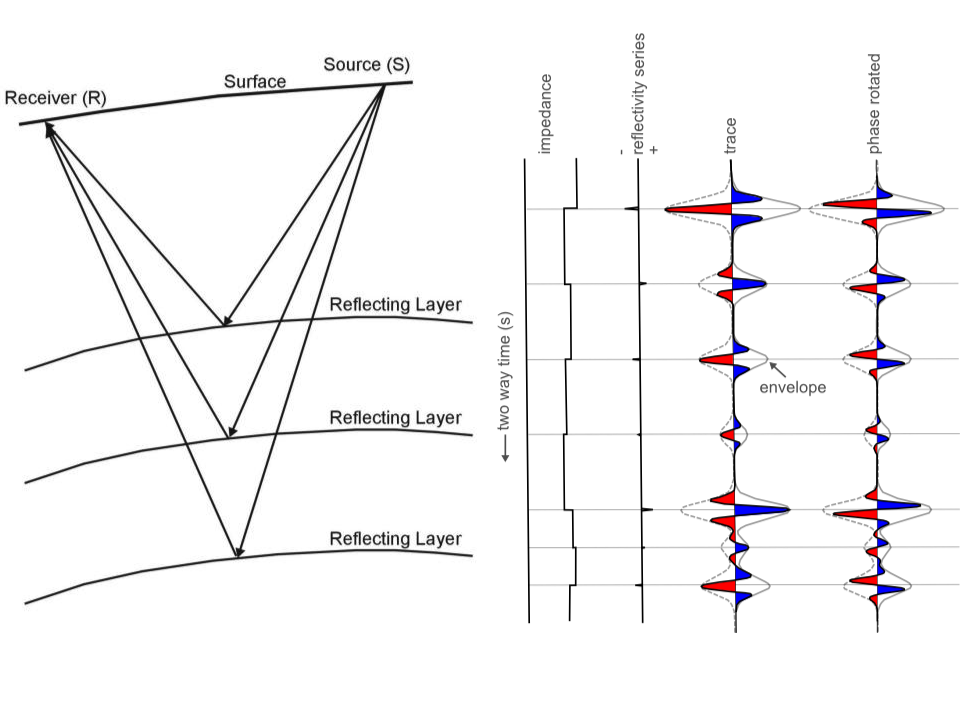
\includegraphics[scale=0.4]{figures/seismic_reflection_principal.png}
\caption{Reflection Seismology \cite{seisreflectionepa} \cite{seisreflectionagile}}
\label{seismic_reflection}
\end{figure}

\section{Big Data Challenge}

The most famous definition of big data, comes from Gartner analyst Doug Laney, specifies the 3Vs characteristics: volume, velocity and variety \cite{demauro2016}. By which volume means the amount of data, velocity stands for the real-time speed of data in and out, and variety is the range of data types and sources. As mentioned in previous section,  the burst increase of volume size, high-speed real-time streaming data from sensors, and various types of structured, unstructured and semi-structured data coming from different stages of seismic data processing all together matches the 3Vs definition. It determines seismic data is costly to store, access and manage in traditional methodology. Therefore, new technology should be adopted to address these problems appropriately.

As the popularity of big data topic grows, there are more and more choices in big data market and open source communities. For instances, Apache Hive and HBase provide the scalable and distributed database solutions,  Apache Storm is capable of handling real-time computation and Apache Kafka is a good choice if users are looking for a distributed streaming platform. These projects provide variety of big data solutions. 

However, all of these big data platforms are designed for general purpose applications and focus on distributing the data, computation and IO overloads. Most MapReduce based framework do not have, or only have limited communication mechanisms between different maps, which is important to resolve the data and logical dependence problems in many complex applications. When it comes to the field of  seismic data processing and analysis, the problem is more complicated. Since most scientists and researchers in petroleum industry do not have big data related knowledge or even computer science background, how to hide parallelism from them and let them easily deploy their works on new platform is a big challenge for all the researchers.

\section{Hadoop File System}

Since Google released its white paper series of big data processing technologies in 2004, the landscape of big data development has been changed profoundly. Many big data projects were inspired and developed based on MapReduce and Google File System framework. Hadoop and Spark is two most widely used open source big data solutions for many business and industry applications in recent years. 

A year after the publication of MapReduce and Google File System framework, Doug Cutting and Mike Cafarella created an open source project Apache Hadoop, which has been utilized in lots of industries to facilitate the works with big volume, variety and velocity of structured and unstructured input datasets \cite{bigdatahistory}. Apache Hadoop consists of Hadoop Distributed File System (HDFS) and MapReduce \cite{ApacheHadoop}.  

Since distributed file system is fundamental to many main stream big data platforms, as it is able to store data across number of storage devices of a cluster, Hadoop Distributed Filesystem becomes one of the most popular Apache subprojects. Originally, HDFS was designed and built for the Apache search engine project Nutch as the file storage infrastructure \cite{ApacheHadoop}. Compare to traditional file system which holds sequential data on one device, HDFS provides far better scalability and support for parallel IO processing mode.

There are some most significant differences that distinguish HDFS from other distributed file systems. First, the high fault-tolerance makes HDFS is able to deployed on low-cost hardware. The high IO throughput access to distributed dataset of HDFS facilitates the applications that have large data sets. Also, HDFS provides streaming access to file system data which is unavailable in conventional POSIX file systems.  

The architecture of a single NameNode and multiple DataNodes in a cluster simplifies the structure of the system. HDFS cluster runs in master-slave mode.  It consists of a single NameNode, the master server which manages the filesystem namespace and the access to distributed datasets, and there are multiple DataNodes, which manage the data storage on the working nodes. HDFS manages the filesystem namespace which enable the general file-form data storage. Files are split into multiple blocks which are saved in multiple DataNodes. The NameNode manages the mapping of data distributions on the DataNodes, and provides general file operations such as open, close, and rename etc. It sends instructions to DataNodes, which perform the related operations on the data blocks and serve the requests of data accessing. Figure \ref{HDFSArch} shows the NameNode-DataNodes architecture of Apache Hadoop File System.

\begin{figure}[h]
\centering
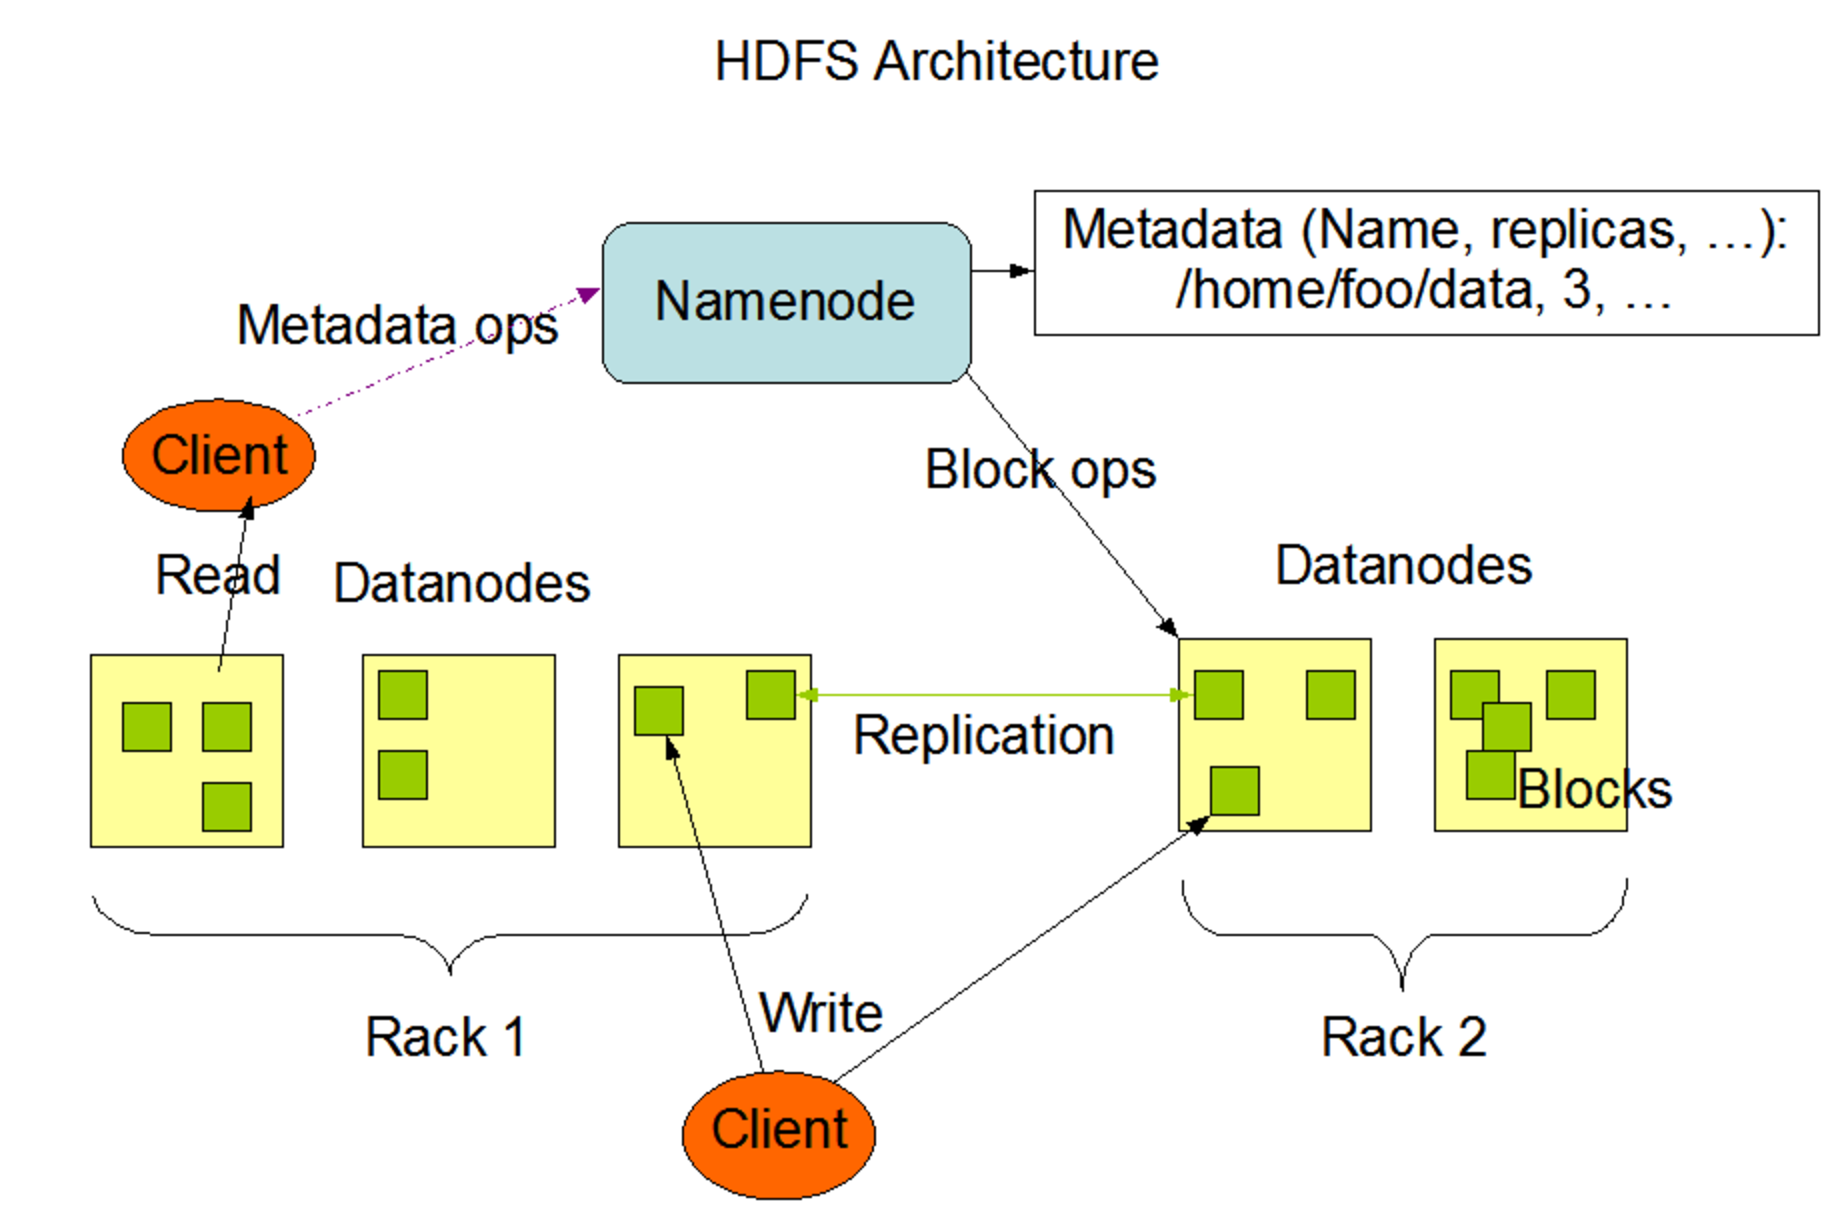
\includegraphics[scale=0.4]{figures/HDFSArch.png}
\caption{The Architecture of Hadoop File System \cite{ApacheHadoop}}
\label{HDFSArch}
\end{figure}

\section{Spark}

The open source big data project Apache Spark provides programmers with an application programming interface centered on a data structure called the resilient distributed dataset (RDD), a fault-tolerant collection of elements that can be operated on in parallel \cite{ApacheSpark}. Since Spark itself does not provide distributed file system, it is usually installed on top of Hadoop, by which Spark could utilize HDFS interface to handle distributed data storage and access. 

The most different part between Hadoop and Spark is the parallel processing interface. MapReduce writes the result back to the storage after each reduction, while Spark utilizes RDD to handle most its operations and result in memory. This leads to up to100 times performance improvement compare to Hadoop in certain circumstances \cite{ApacheSpark}. Another advantage of Spark is it provides more advanced features such as real-time streaming processing interface and machine-learning library.

\subsection{Resilient Distributed Dataset}

Resilient Distributed Dataset (RDD) is distributed data collection with high fault-tolerance and can be accessed and operated in parallel. A RDD can be generated in two way, transforming an existed RDD to a new RDD, or importing the data stored in file storage system. Although Spark supports data loading from both traditional and distributed file system, it is designed for performing on the latter one for the high performance and parallelism. Spark supports any data source providing the Hadoop input format, such as HDFS and HBase \cite{ApacheSpark}.



\subsection{Programming Model}


%%%%%%%%%%%%%%%%%%%%%%%%%%%%%%%%%%%%%%%%%%%%%%%%%%%%%%%
%\subsection{Subsection}

%A table example is going to follow.

%\begin{table}[H]
%\centering
%\caption{This is a table template}
%\begin{tabular}{|l|c|c|c|c|c|}
%\hline
%Product & 1 & 2 & 3 & 4 & 5\\
%\hline
%Price & 124.- & 136.- & 85.- & 156.- & 23.-\\
%Guarantee [years] & 1 & 2 & - & 3 & 1\\
%Rating & 89\% & 84\% & 51\% & & 45\%\\
%\hline
%\hline
%Recommended & yes & yes & no & no & no\\
%\hline
%\end{tabular}
%\label{tab:template2}
%\end{table}
%\subsubsection{This is a subsubsection}



%%%%%%%%%%%%%%%%%%%%%%%%%%%%%%%%%%%%%%%%%%%%%%%%%%%
%
%  New template code for TAMU Theses and Dissertations starting Fall 2012.  
%  For more info about this template or the 
%  TAMU LaTeX User's Group, see http://www.howdy.me/.
%
%  Author: Wendy Lynn Turner 
%	 Version 1.0 
%  Last updated 8/5/2012
%
%%%%%%%%%%%%%%%%%%%%%%%%%%%%%%%%%%%%%%%%%%%%%%%%%%%
%%%%%%%%%%%%%%%%%%%%%%%%%%%%%%%%%%%%%%%%%%%%%%%%%%%%%%%%%%%%%%%%%%%%%%
%%                           SECTION III
%%%%%%%%%%%%%%%%%%%%%%%%%%%%%%%%%%%%%%%%%%%%%%%%%%%%%%%%%%%%%%%%%%%%%

\chapter{\uppercase{Related Work}}

%Traditonal Workflow
%Data Interpretation
%Data Visualization
%Faults Prediction
%Attributes Computation
%Execution
%HPC
%IO Scalability
%Ease to use

Although various motivations exist in petroleum companies to adopt big data solutions to improve efficiency and reduce cost, only a few of them have deployed big data solutions. This situation may due to some technique barriers such as lack of technology knowledge, big data solution are not applicable in some steps of traditional workflow, and the cost and risk to convert legacy software to fit new platform etc. Moreover, there are lots of concerns of business-wise, such as the cost of infrastructure and data security issue (business or political restrictions on data accessing). 

In \cite{bigdatatooil}, it concludes that the applications of big data analytics in the petroleum industry are still in experimental stage. Only a few companies have applied the Big Data techniques on their workflows, and most of these innovations are developed by oil \& gas service contracting companies such as Schlumberger and Halliburton, as well as some IT solution providers like IBM and Microsoft: \\

\begin{enumerate}
  \item Chevron proof-of-concept adopted Apache Hadoop (IBM BigInsights) for seismic data processing;
  \item Shell piloting Apache Hadoop in Amazon Virtual Private Cloud (Amazon VPC) for seismic sensor data;
  \item Cloudera Seismic Hadoop integrated Seismic Unix with Apache Hadoop;
  \item PointCross Seismic Data Server and Drilling Data Server utilizing Apache Hadoop / NoSQL;
  \item University of Stavanger data acquisition performance research used Apache Hadoop.
\end{enumerate}



%%%%%%%%%%%%%%%%%%%%%%%%%%%%%%%%%%%%%%%%%%%%%%%%%%
%
%  New template code for TAMU Theses and Dissertations starting Fall 2012.  
%  For more info about this template or the 
%  TAMU LaTeX User's Group, see http://www.howdy.me/.
%
%  Author: Wendy Lynn Turner 
%	 Version 1.0 
%  Last updated 8/5/2012
%
%%%%%%%%%%%%%%%%%%%%%%%%%%%%%%%%%%%%%%%%%%%%%%%%%%%
%%%%%%%%%%%%%%%%%%%%%%%%%%%%%%%%%%%%%%%%%%%%%%%%%%%%%%%%%%%%%%%%%%%%%%
%%                           SECTION IV
%%%%%%%%%%%%%%%%%%%%%%%%%%%%%%%%%%%%%%%%%%%%%%%%%%%%%%%%%%%%%%%%%%%%%

\chapter{\uppercase{Design}}

The main goal of Seismic Data Analytics SDK is to implement a distributed software development toolkit to enable scalable storage, computation and analytics for big seismic volume datasets. This chapter will introduce the software architecture design and main functionalities of this toolkit.

\section{Software Architecture Design}

Seismic Data Analytics SDK is built upon Apache Hadoop and Spark. Figure \ref{sdk_swstack} shows the software stack of a workable seismic data analytics platform. In this diagram, the gray part is the OS layer, the elements with green color stands for the infrastructure layer of this big data platform, and on top of that, SDK layer consists of the components with blue color. At the bottom of the infrastructure layer, there is Hadoop Distributed File System (HDFS) that stores the big seismic data files by utilizing the large number of local disks. The Cassandra as a NoSQL database is also used to store  seismic data, intermediate results and meta data. YARN and Mesos are used for resources management. Apache Spark is the data distribution and parallel execution engine based on the innovative idea of Resilient Distributed DataSets (RDD) concept. MLLib is included in the Spark as the machine learning package to enable machine learning based data analytics algorithms. OpenCV is the widely used image processing package that is used to provide image processing capability. Breeze is the numerical processing package including linear algebra, signal processing, statistics, and other numerical computation and optimizations written in Scala. We have developed the seismic data RDD on top of Spark as the base distributed seismic datasets to enable parallel operations and machine learning algorithms. Geophysicists and data scientists can use  Seismic Data Analytics SDK to develop their own algorithms and leverage the capability of Apache Spark, as well as image processing, numerical computation, and deep learning packages.

\begin{figure}[h]
\centering
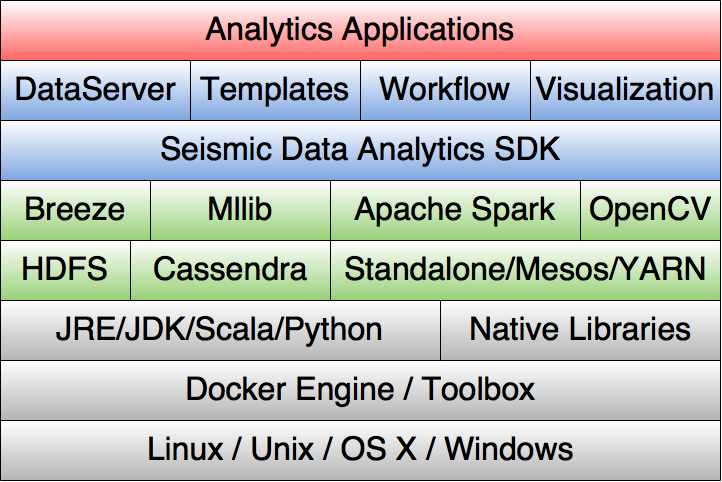
\includegraphics[scale=0.4]{figures/sdk_swstack.png}
\caption{Software Stack of Seismic Data Analytics Platform}
\label{sdk_swstack}
\end{figure}

Figure \ref{sdk_framework} simplifies the development efforts for scalable and distributed computing and analytics of seismic datasets. It is built on top of the Apache Hadoop and Spark. The Hadoop provides a distributed file system(HDFS) and resource management system (YARN and Mesos), while Spark provides a high-level distributed data representation via Resilient Data Sets (RDD) and a data-parallelism execution engine. Seismic Data Analytics SDK provides configurable data distribution fashions for seismic volume data, as well as a configurable parallel execution interface to simplify the parallel programming efforts. Based on the functionality of SDK, we developed two useful utilities, parallel templates and data server, to facilitate SDK for users to easily deploy their applications. Moreover, since Hadoop and Spark provide faults tolerance and task scheduling utilities, the toolkit inherits from them to provide fault tolerance and dynamic task scheduling for better reliability and task management.

\begin{figure}[h]
\centering
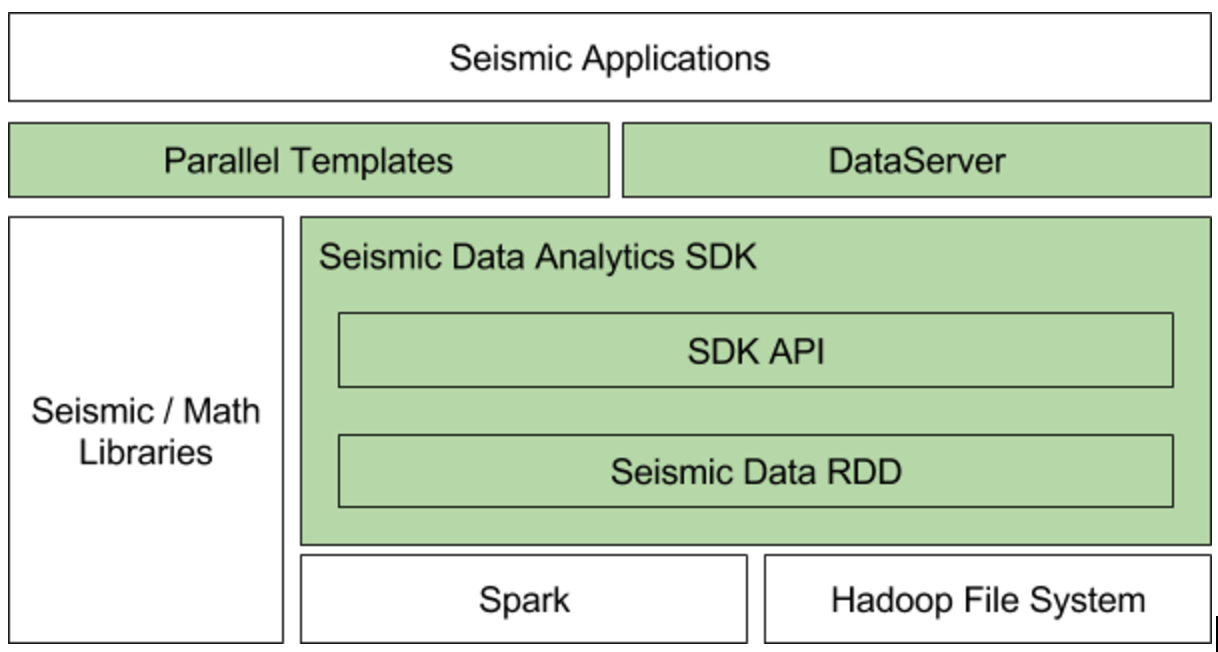
\includegraphics[scale=0.6]{figures/sdk_framework.png}
\caption{Framework of Seismic Data Analytics SDK}
\label{sdk_framework}
\end{figure}


\section{Interfaces and Functionalities}

Figure \ref{sdk_interface} shows the main functionalities of Seismic Data Analytics SDK, including data loading/saving, configurable distribution, data accessing, 3D transpose and user-defined function mapping. It provides a single public class \emph{SeismicVolume}, which integrates all the APIs of SDK. Developers are able to create \emph{SeismicVolume} instances for specified seismic dataset, access data by configurable grain, perform 3D transposing and apply user function to the distributed data instance, and finally save the result to distributed file system through save API. The invalid input data format include 3D binary data and SEG-Y file \cite{SEGDREV21} which is one of the most widely used industrial standard format for seismic data.

\begin{figure}[h]
\centering
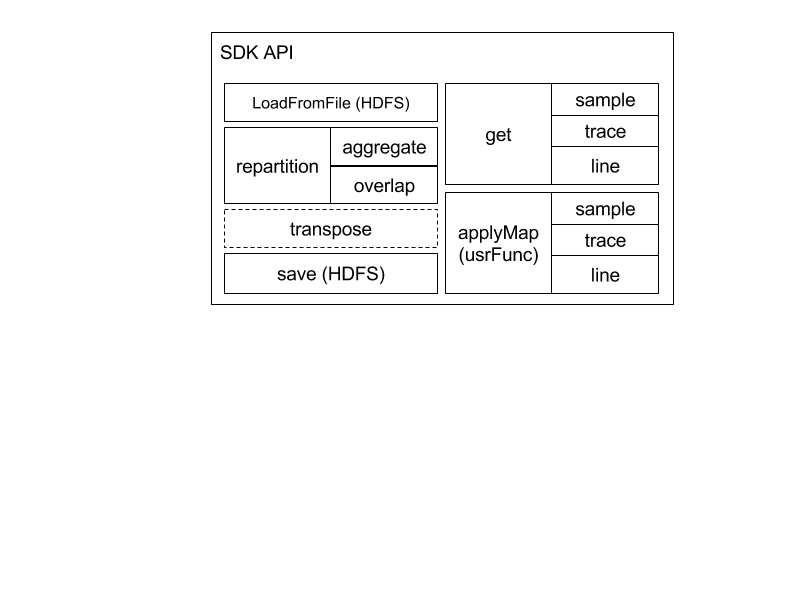
\includegraphics[scale=0.6]{figures/sdk_interface.png}
\caption{Main APIs of Seismic Data Analytics SDK}
\label{sdk_interface}
\end{figure}

\section{Programming Language}

The host programming language of Seismic Analytics SDK is Scala, and the applications can be developed in Java. Scala (The acronym for Scalable Language), an object-oriented and functional language, provides great scalability in developing safe and high efficient multi-threaded programs \cite{ScalaOrg}. The most important reason of using Scala as host language is it's also the native host language of Apache Spark. It means Scala is the most efficient programming language of this project. Moreover, Scala runs on the JVM which determines it can be freely integrated with Java and Java libraries and tools are also available. Since Scala compiler contains a subset of a Java compiler, Seismic Analytics SDK allows users who are not familiar with Scala can develop their applications in Java. This feature makes it possible for developers to port the legacy Java applications to Seismic Analytics SDK without putting extra efforts on learning a new programming language.

%%%%%%%%%%%%%%%%%%%%%%%%%%%%%%%%%%%%%%%%%%%%%%%%%%
%
%  New template code for TAMU Theses and Dissertations starting Fall 2012.  
%  For more info about this template or the 
%  TAMU LaTeX User's Group, see http://www.howdy.me/.
%
%  Author: Wendy Lynn Turner 
%	 Version 1.0 
%  Last updated 8/5/2012
%
%%%%%%%%%%%%%%%%%%%%%%%%%%%%%%%%%%%%%%%%%%%%%%%%%%%
%%%%%%%%%%%%%%%%%%%%%%%%%%%%%%%%%%%%%%%%%%%%%%%%%%%%%%%%%%%%%%%%%%%%%%
%%                           SECTION IV
%%%%%%%%%%%%%%%%%%%%%%%%%%%%%%%%%%%%%%%%%%%%%%%%%%%%%%%%%%%%%%%%%%%%%

\chapter{\uppercase{Implementation}}

\section{Seismic Volume Data Loading, Distribution and Saving}

As mentioned in chapter 2, seismic 3D volume data is a collection of estimated property values of the Earth's subsurface, obtained through seismic reflection survey and organized in 3D spacing form. It is widely used in energy companies for geophysics analysis, which could conduct more accurate subsurface exploration and exploit. As shown in Figure \ref{seisdata}, the seismic volume data is defined through 3 different directions in 3D space: inline, crossline and timeline. The industry usually stored the data slice by slice along crossline direction and each slice is a inline section, which is also the default data organization format of Seismic Data Analytics SDK. In this case, each inline slice is a single split of the whole dataset.

\begin{figure}[h]
\centering
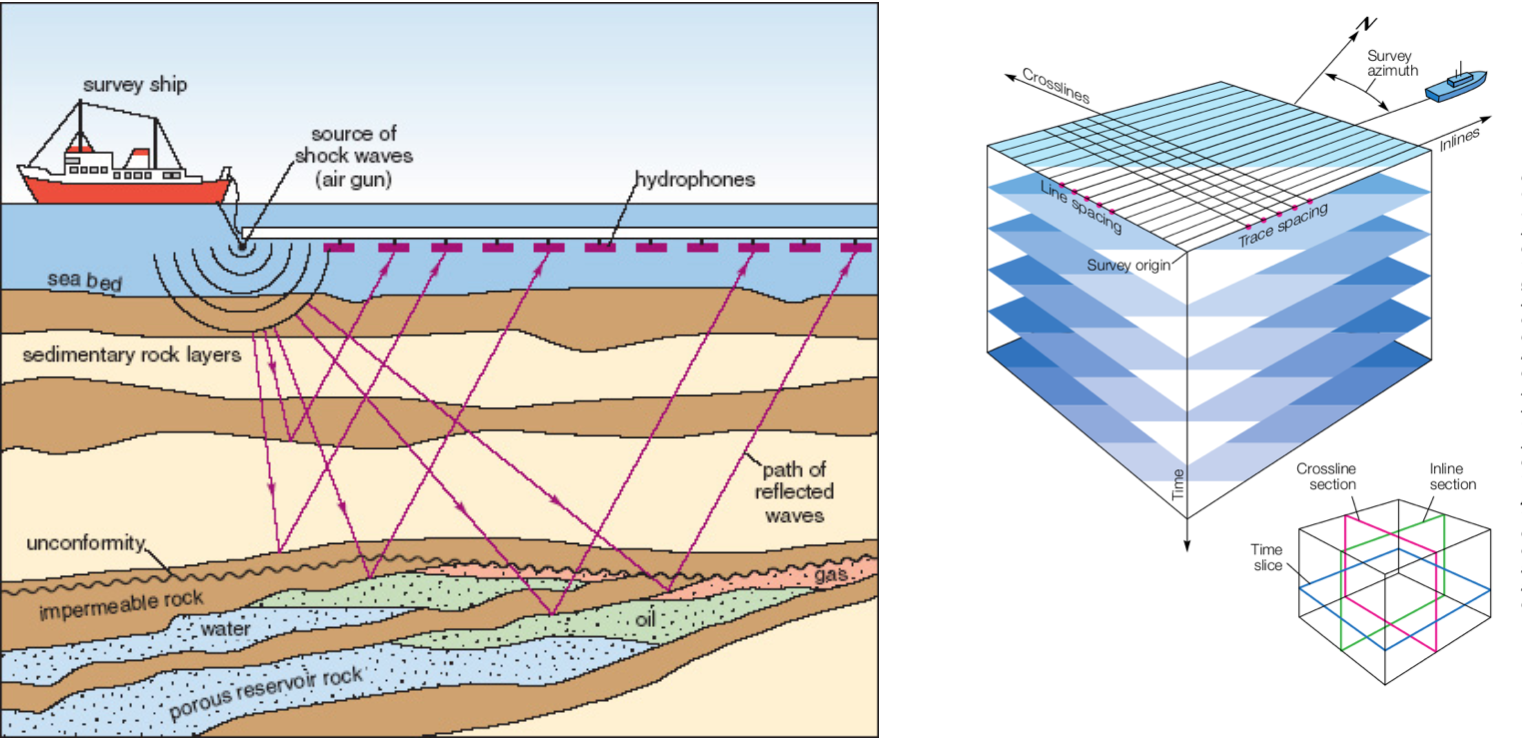
\includegraphics[scale=0.6]{figures/seisdata.png}
\caption{Seismic Volume Data \cite{seisinline}}
\label{seisdata}
\end{figure}

The public class \emph{SeismicVolume} provides an API \emph{loadFromFile()} to load seismic data from HDFS and distribute them over Spark RDD according to users configurations. This API generates a \emph{SeismicVolume} instance which contains a SeismicRDD with float/byte as internal binary data types. The SeismicRDD is a derived class from Spark RDD class with a variety of distributed fashions of seismic volume data. In addition, it also provides some optional parameters for advanced users who have already familiar with distributed system to specify the advanced data distribution fashions. 

Figure \ref{datadist} shows the flow of distributing an seismic volume file through the Hadoop filesystem and Spark RDD. It assumes the file has already been uploaded to Hadoop file system, which is able to support the distributed IO accessing for Spark to load data in parallel. After users get the  \emph{SeismicVolume} instance of a specified file,  all Spark RDD operations can be applied to the inside SeismicRDD object. Utilizing the RDD methods provided by Spark, developer could perform various of data operations and calculations on the dataset in parallel. By default, SDK distributes the volume in inline format slice by slice, which means each partition contains one single inline slice. The distribution direction could also be configured to crossline/timeline by given parameters in other APIs, this function will be present in the following Volume Data 3D Transposing section. Users could configure the slices count of each distribution to manage the data distribution grain, thus to efficiently tuning the performance of applications.

\begin{figure}[h]
\centering
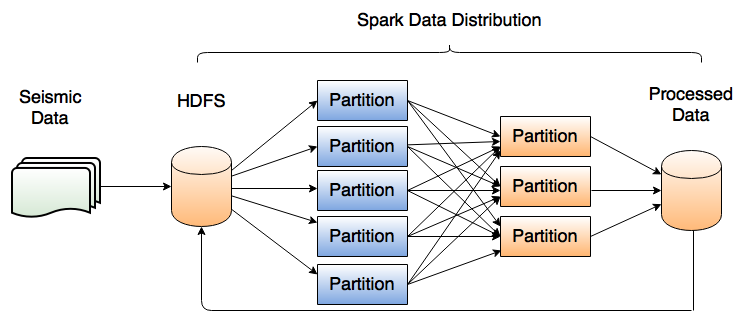
\includegraphics[scale=0.6]{figures/datadist.png}
\caption{Seismic Volume Data Distribution Flow}
\label{datadist}
\end{figure}

\emph{SeismicVolume} class also provides \emph{save()} API to allow users to store the data of SeismicRDD back to the HDFS. Although this operation is not recommended since it could introduce performance issues caused by data shuffling, it is still necessary when users need to backup the runtime data or apply the runtime data to traditional sequential workflows.


\section{Volume Data Accessing}

\begin{figure}[h]
\centering
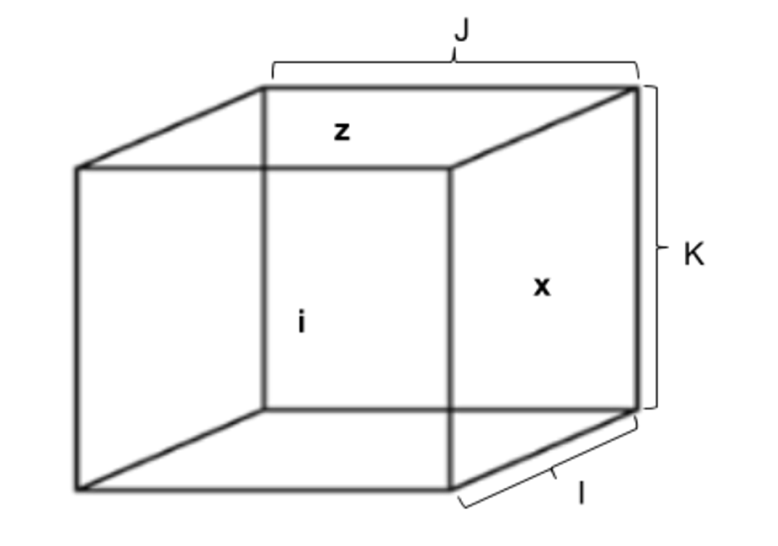
\includegraphics[scale=0.6]{figures/VolumeDim.png}
\caption{Seismic Volume Data Dimensions}
\label{VolumeDim}
\end{figure}

Seismic Data Analytics SDK allows users to to access any slice/trace/sample data in any direction of the volume through \emph{SeismicVolume} APIs \emph{getLine(direction:Int, idx:Int):Array[T]}, \emph{getTrace(dir:Int, i:Int, j:Int):Array[T]} and \emph{getSample(i:Int, j:Int, k:Int):T}. 

For the convenience of addressing the data organization, we defined the three dimension of seismic volume as I (Dimension of inline slices), J (Dimension of crossline slices) and K (Dimension of timeline slices), as shown in Figure \ref{VolumeDim} and Figure \ref{VolumeTrans}. Users can specify any one of I, J and K directions to access data for visualization or computation purpose.  Figure \ref{code_load_access} shows the example of accessing seismic data by \emph{getLine(direction:Int, idx:Int):Array[T]} API. The first parameter of \emph{getLine}, which has three possible direction values(1 stands for I, 2 stands for J and 3 means K), specifies the direction users want to extract the data slice out of.  The second parameter is the index number of the target slice in specified direction.

\begin{figure}[h]
\centering
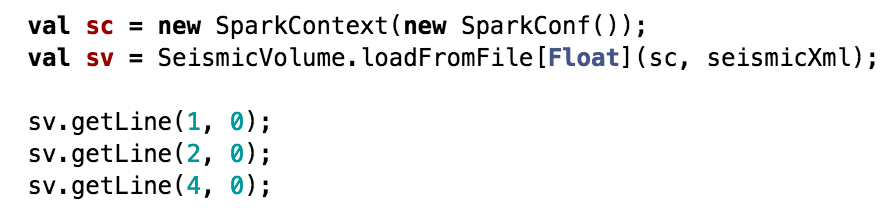
\includegraphics[scale=0.8]{figures/code_load_access.png}
\caption{Example Code of Accessing Data Slice in SeismicVolume}
\label{code_load_access}
\end{figure}


Since Spark does not provide arbitrary data access, the APIs used IndexedRDD, a more efficient key-value management than native Spark API \cite{IndexedRDD}, to implement and speedup queries of slice/trace/sample data from any distributions to the master node.


\section{Volume Data 3D Transposing}

Since the volume data could only be stored in file following one specific direction(I, J or K), developer could not access slices of the other two directions directly. In traditional solutions, if users need data in other directions, organized as cross-line slice or time-line slice, the data fetching program must perform lots of seek operations between different file offsets to collect the data of a single cross-line or time-line slice. This tedious procedure will dramatically slow down the whole software performance. To resolve this problem and to achieve reasonable performance, SDK handles the transposing of the 3D volume data inside the \emph{SeismicVolume} APIs and caches all three directions format SeismicRDD in \emph{SeismicVolume}.

To explain the implementation clearly, we denote the seismic volume data as shown in Figure \ref{VolumeDim}, in which i means I slice, x means J slice and z stands for K slice. The data is stored in iSlices format by default. To resolve the transposing problem in each distribution evenly, we split the volume to I of iSlices and distribute them over SeismicRDD. Each iSlice is a 2D matrix. As shown in Figure \ref{VolumeTrans}, each iSlice matrix consists of J of iTraces which have the length of K. An iSlice matrix could be iterated iTrace by iTrace. Since in 3D spacing, each iTrace is also the trace of xSlice, for example, the iTraces(0) is the xTrace of the 0th xSlice, the iTraces(1) is the xTrace of 1st xSlice, etc. 

As mentioned in previous section, the default distribution of \emph{SeismicVolume} splits the data slice by slice. To transpose the volume data organization to different direction,  first we need to split the slice data partitions to number of smaller trace partitions and index them by trace index number. This process can be achieved by using \emph{flatmap()} operation of Spark RDD. Figure \ref{RDDFlatmap} demonstrates how it splits the data partitions to more fine grain partitions. We apply a map function to \emph{flatmap()} API to index all iTraces of the volume. The new index is combined by index of iTrace and index of iSlice. After indexing the trace map, we got a volume RDD with new (iTraceIndex)(iSliceIndex) index as the key and trace data as the value.

\begin{figure}[h]
\centering
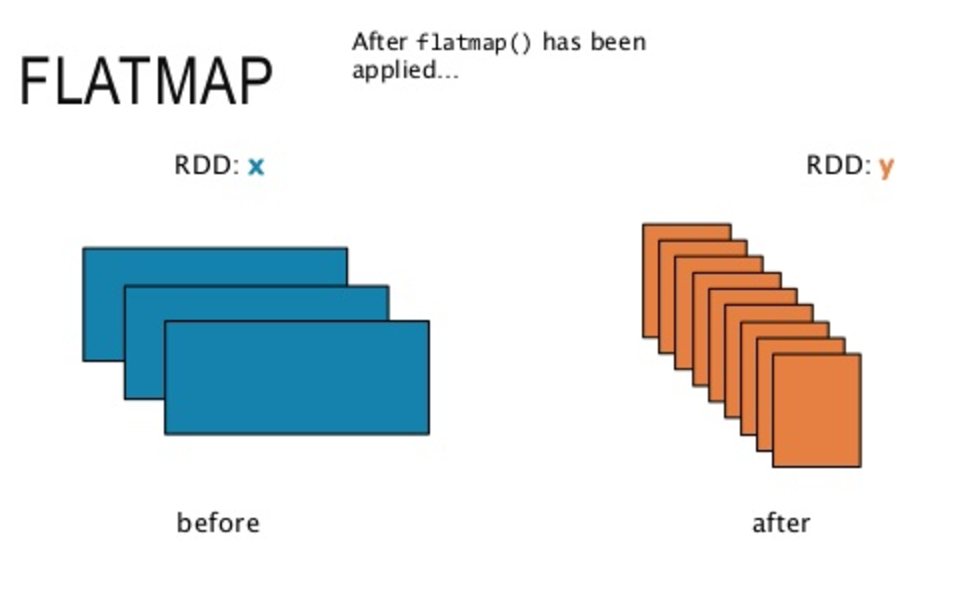
\includegraphics[scale=0.8]{figures/RDDFlatmap.png}
\caption{Flatmap Operation of Spark RDD}
\label{RDDFlatmap}
\end{figure}


As shown in Figure \ref{VolumeTrans}, to get a xSlice, the next step is to group all the traces with the same iTraceIndex by utilizing the \emph{groupByKey} operations of Spark RDD. As shown in Figure \ref{RDDGroup}, this API groups all the data splits sharing the same key feature to a new data partition. After grouping, the xSlices data collection is generated in the new SeismicRDD distribution map. To organize them as a xSlices volume, all we need to do is sorting them by iTraceIndex. So far, the data in requested direction has already been stored in the \emph{SeismicVolume} instance, therefore users could access and manipulate seismic data in any direction by specifying the direction parameter of related \emph{SeismicVolume} APIs.

\begin{figure}[h]
\centering
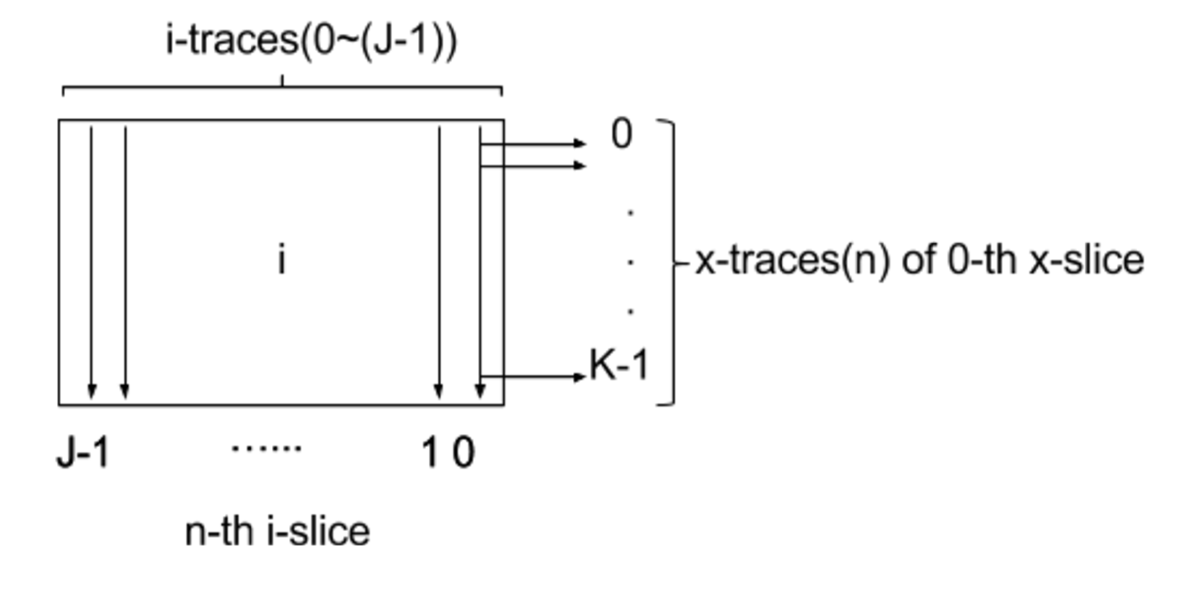
\includegraphics[scale=0.6]{figures/VolumeTrans.png}
\caption{The Indexing for Resolving 3D Transposing Problem}
\label{VolumeTrans}
\end{figure}

\begin{figure}[h]
\centering
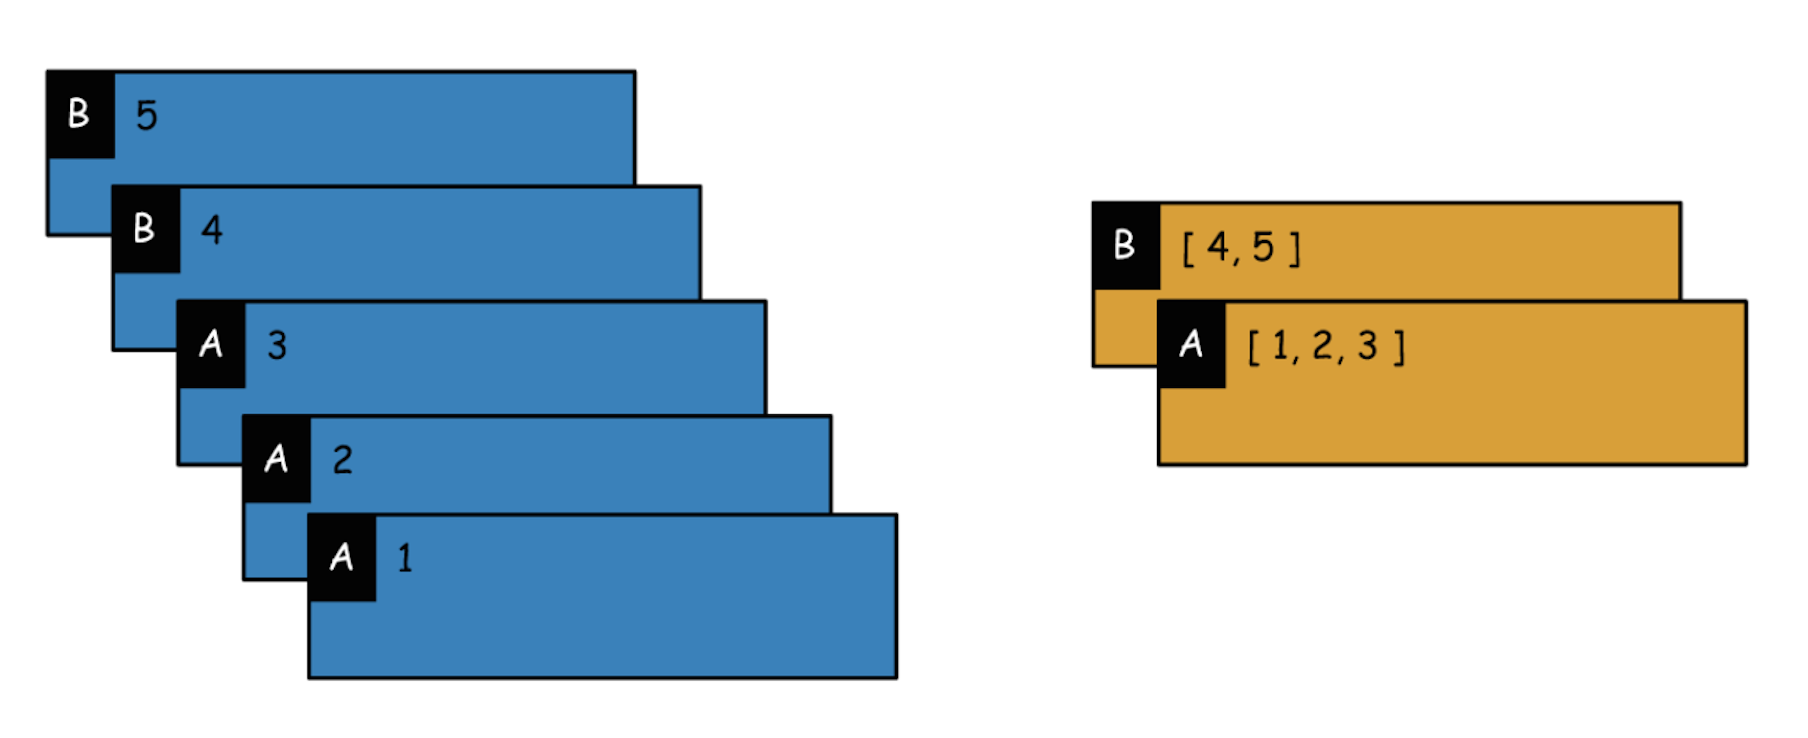
\includegraphics[scale=0.4]{figures/RDDGroup.png}
\caption{GroupByKey Operation of Spark RDD}
\label{RDDGroup}
\end{figure}


\section{Repartition}

Users need a way to configure the data partition size and partitions number, since they need to efficiently tune the granularity of the distributed process to achieve better performance. By default, as shown in Figure \ref{DefDist}, SDK distributes the volume in one specific direction slice by slice. In this case, each slice is a single split of the whole dataset. However, it will cause performance problems for some applications if we only support one distribution. For an instance, the transposing solution as mentioned in previous section needs to do lots of data exchanges between different data splits for the \emph{group} operation to shuffle the dataset to expected arrangement. Since data shuffle in Spark RDD relies on lots of physical storage access and network transmissions in each worker node, it will become the bottleneck of the transposing performance if the number of partitions is too big. Obviously, to speedup the transposing operation, users need to reduce the number of partitions thus to reduce the data communications between worker nodes.

Developers can change the distribution layout to the aggregated and overlapped fashions as shown in Figure \ref{Aggregation} and Figure \ref{Overlap} by utilizing the \emph{SeismicVolume} API :

\emph{repartition(planesPerMap:Int,overlapPlanes:Int):SeismicVolume[T]}.


\subsection{Aggregation}

\begin{figure}[h]
\centering
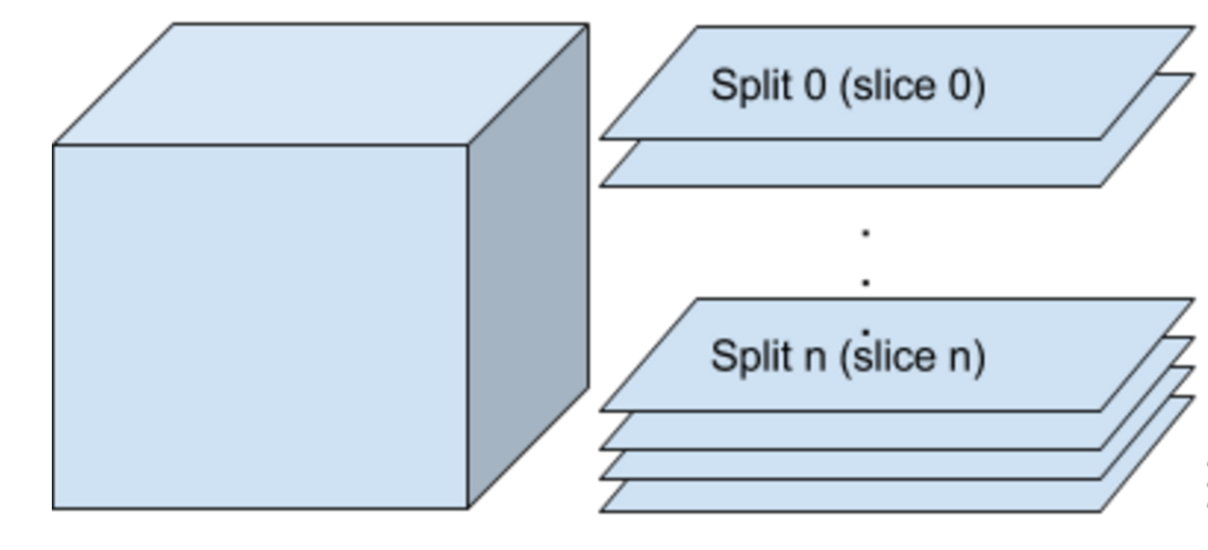
\includegraphics[scale=0.6]{figures/DefDist.png}
\caption{Default Distribution Fashion of Volume, planesPerMap=1, overlap=0}
\label{DefDist}
\end{figure}

As shown in Figure \ref{Aggregation}, aggregated data distribution could be achieved by utilizing the RDD group operations we mentioned in Volume Data 3D transposing section. The solution of this problem is to re-indexing all the slices in parallel through RDD map function by arranging an unique key to multiple data splits, then use RDD \emph{groupByKey()} API to repartition the dataset. An aggregated dataset could have multiple slices in a single data split.

\begin{figure}[h]
\centering
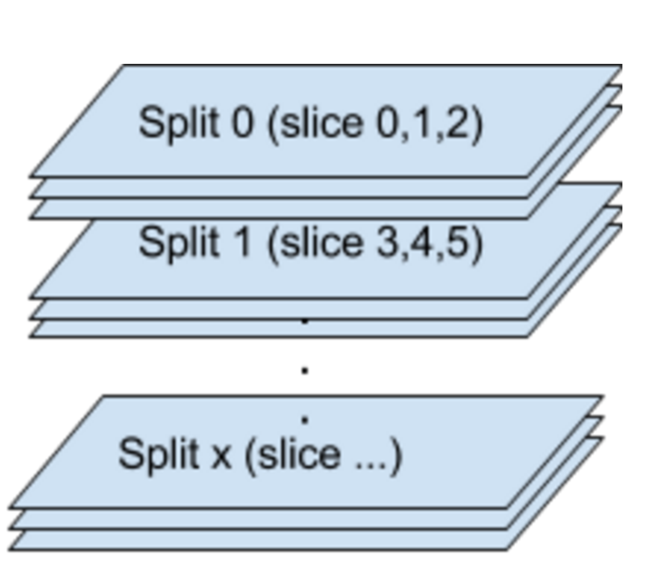
\includegraphics[scale=0.6]{figures/Aggregation.png}
\caption{Aggregated Distribution of Volume, planesPerMap=3, overlap=0}
\label{Aggregation}
\end{figure}

\subsection{Overlapping}

The \emph{repartition()} method not only lets users change the size of distributed splits, more powerfully, it allows developer to set the overlapped data areas between splits and to access the overlapped parts in each split. Practically, some applications may have strong data dependences in their logic which is very hard to parallelize the solutions. For example, the stencil computation needs lots of data communications between neighbor units in each step, which is impossible to run it in parallel with other MapReduce frameworks. 

To resolve this problem, \emph{repartition()} API generates the head and tail boundaries RDD on top of the aggregated SeismicRDD and indexing them according to the related partition numbers. Finally, the boundaries are appended to each related data split through RDD \emph{zip()} API to generate a new \emph{SeismicVolume} instance which contains overlapped SeismicRDD. Figure \ref{boundaryRDD} shows the process of boundary RDD solution.

\begin{figure}[h]
\centering
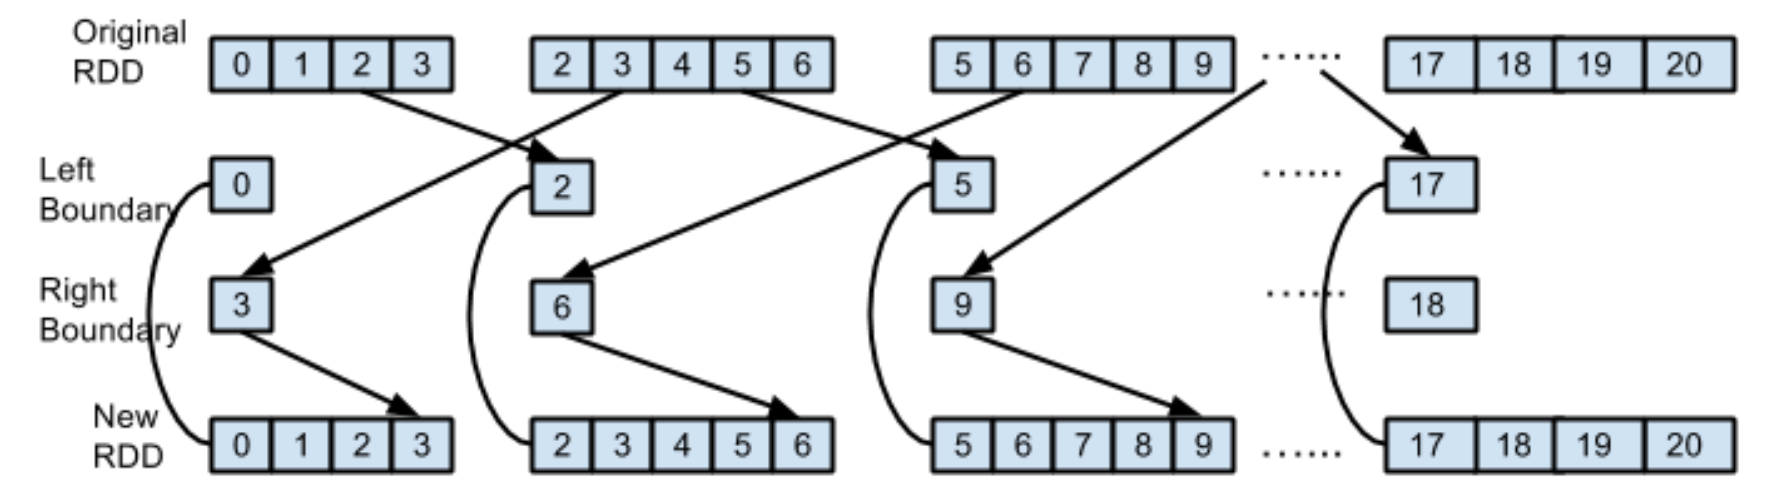
\includegraphics[scale=0.5]{figures/boundaryRDD.png}
\caption{The Boundary RDD Solution of Overlapping Problem}
\label{boundaryRDD}
\end{figure}

\begin{figure}[h]
\centering
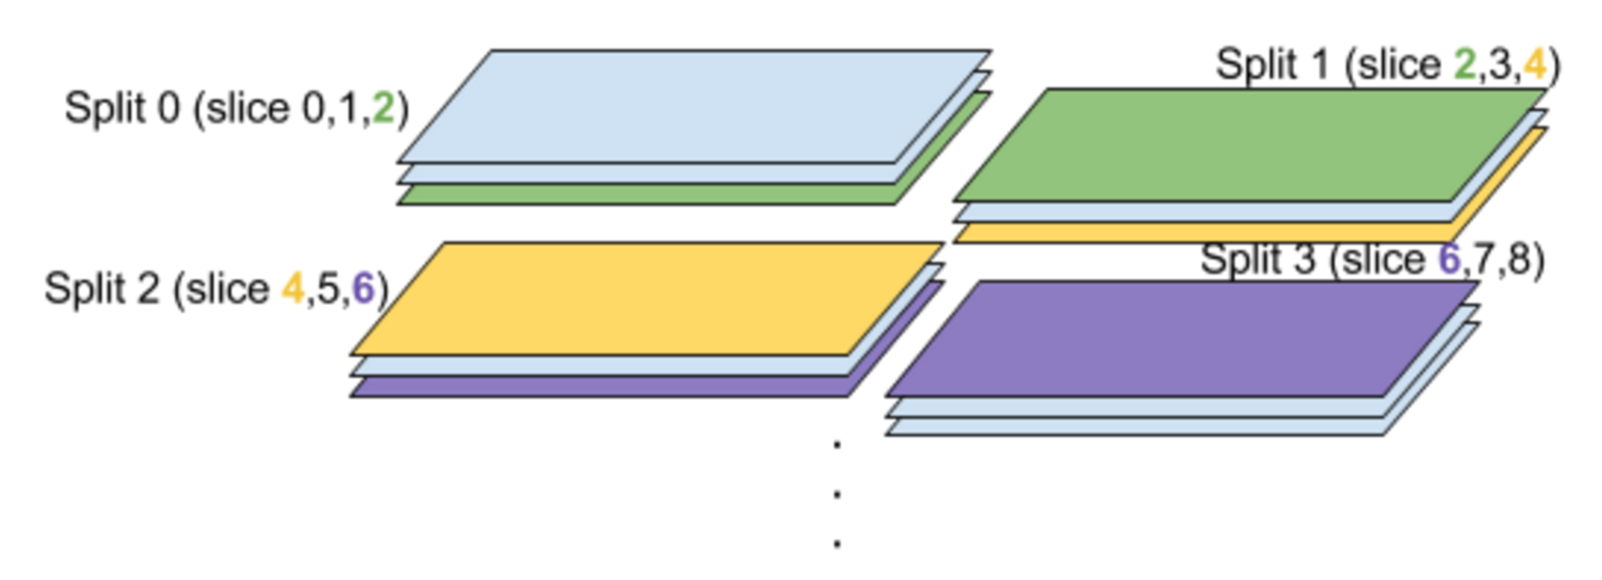
\includegraphics[scale=0.5]{figures/Overlap.png}
\caption{Overlapped distribution of Volume, planesPerMap=1, overlap=1}
\label{Overlap}
\end{figure}

Therefore, this method is not only capable of tuning the performance of distributed tasks, but also simplifies the stencil-style computation requiring neighbor communication, which is not easy to parallelize in MapReduce programming mode. We have developed a more complicated 3D stencil use case with 3D spacing overlapping which will be presented in detail in following Experiments chapter. It could be used for resolving seismic 3D attributes computation problem.


\section{User Defined Function Mapping}

As mentioned in Introduction chapter, one of the project's objective is to provide an easy-to-use solution for geophysicists or data scientists to apply their programs on big data platform without concerning the parallelism and code reconstruction. To achieve this, \emph{SeismicVolume} provides \emph{applyMap()} API to allow developer to apply user-defined functions on any direction of the SeismicRDD in parallel. The user function itself could be written in sequential mode, the SDK execution engine will parallelize it over the cluster.

The prototype of this API is \emph{applyMap(direction:Int, f:(T-U))}. The first parameter \emph{direction} indicates the direction that users would like to apply the function on. The other parameter \emph{f:(T-U)} is a standard spark RDD key-value pairs operation callback function, which feeds the function distributed volume data with key-value forms in parallel. The data length in each key-value function depends on the specified distribution parameters of the target \emph{SeismicVolume}.  Users could apply any operation or computation on any given input data, and an output key-value pairs is required for the return value. This callback function will be executed over the specified data distribution in parallel. After execution, it will generate a new \emph{SeismicVolume} object that containing the processed and distributed output data.  Figure \ref{code_apply} shows the example code of applying an user function to a \emph{SeismicVolume} instance.

\begin{figure}[h]
\centering
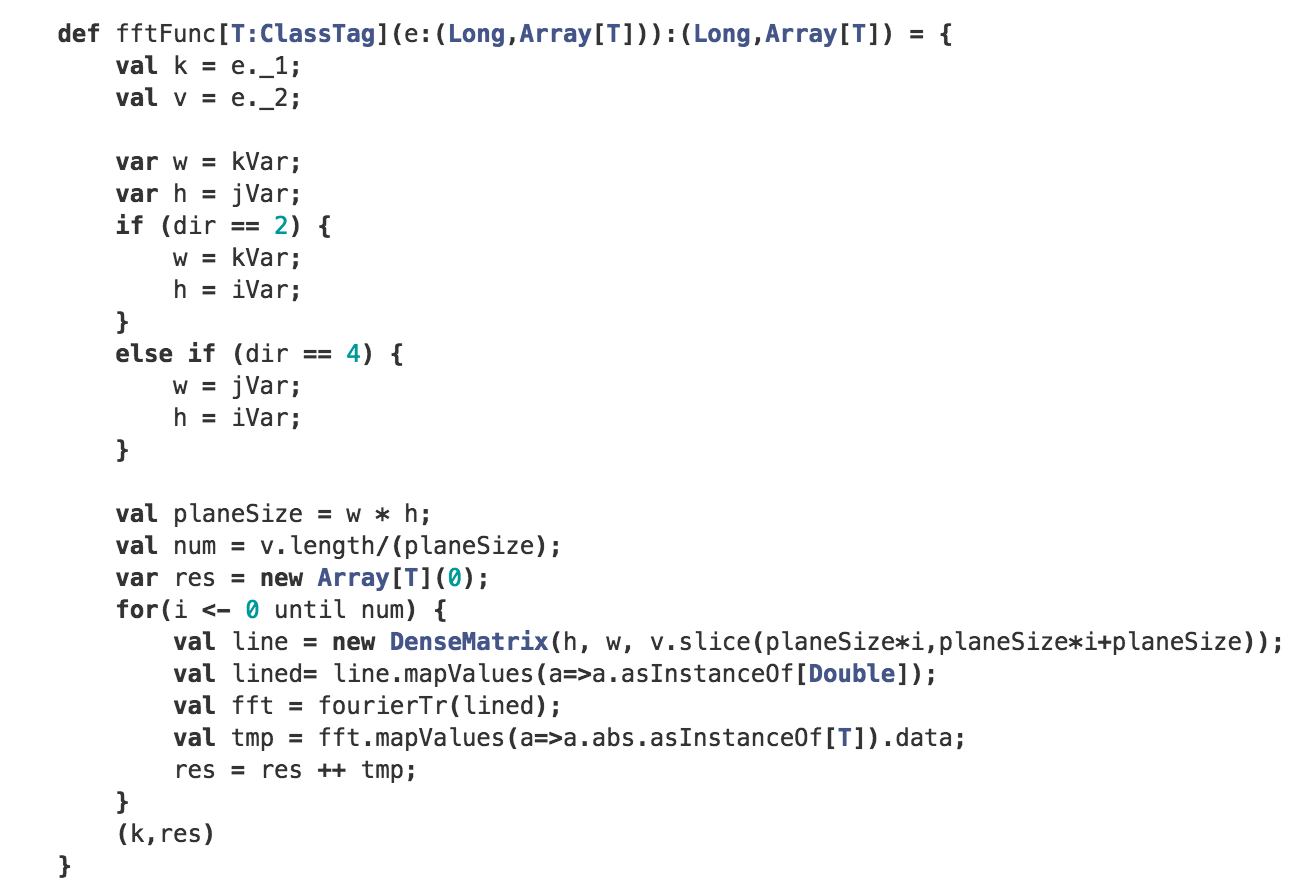
\includegraphics[scale=0.65]{figures/code_apply.png}
\caption{Sample Code for Applying User-defined function in Parallel}
\label{code_apply}
\end{figure}


\section{Parallel Templates}

Data distribution plays an important role in parallel programs to achieve scalable performance. However, most scientists and researchers in petroleum industry do not have enough big data background knowledge to support them to convert their work to Spark applications. To overcome the usability barriers, we developed several parallel templates based on Seismic Data Analytics SDK APIs to make it be easily used by domain algorithm designer other than computer scientists.

These templates defines the data distributions and parallel computation so that users can simply select the right templates for their algorithms without handling the data distribution and parallelism details. Three templates currently include: Trace, Line and Sub-volume. Each template can handle one or more volumes, and will output one or more volumes. Trace template is simple, in which the input is a 2D array (dimension 1 for number of volumes and dimension 2 for 1D trace data), and output is also a 2D array. Line template defines a 3D array as input and a 3D array as output respectively (dimension 1 for number of volumes and dimension 2 for 2D slice data, line is the petroleum terminology). Sub-volume template is a powerful solution to handle data 3D data distribution with overlaps, in which both input and output are 4D array (dimension 1 for number of volumes and dimension 2 for 3D overlapped sub-volume data). The Sub-volume template outputs data without any overlapping. Users can specify parameters about how to distribute data as well as the overlapped areas. 

Figure \ref{code_tmpl_line} shows an example of the Line Template and Figure \ref{code_tmpl_subv} shows the example of Sub-volume Template. Both of them are straight forward and require very few knowledge about parallel computing. The only thing users should be aware of is the distribution grain of input/output data, which is specified in the distribution parameter when users create the template instance. As shown in Figure \ref{code_run_subv}, it demonstrates the execution of an Sub-volume Template instance, in which the distributed input sub-volume size in dimension I and J (for each parallel \emph{proc()} callback function) is set to 26 x 21(The sub-volume size in dimension K is always the complete length of iTrace/xTrace, which is the minimal unit for seismic computation), and the overlapping size is 4 in both I and J direction (Each data split extends to 30 x 25 in I x J). 

\begin{figure}[h]
\centering
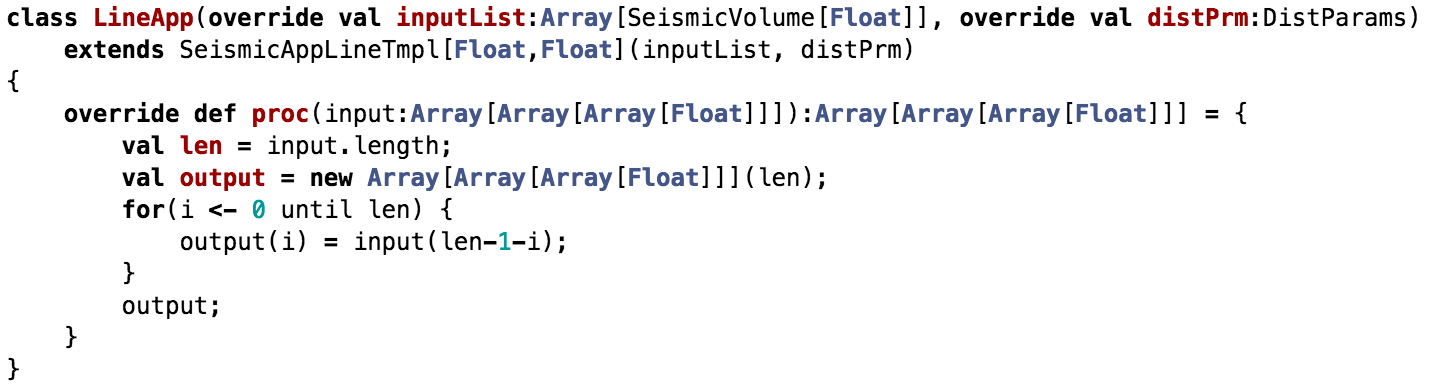
\includegraphics[scale=0.55]{figures/code_tmpl_line.png}
\caption{Sample Code of Line Parallel Template}
\label{code_tmpl_line}
\end{figure}

\begin{figure}[h]
\centering
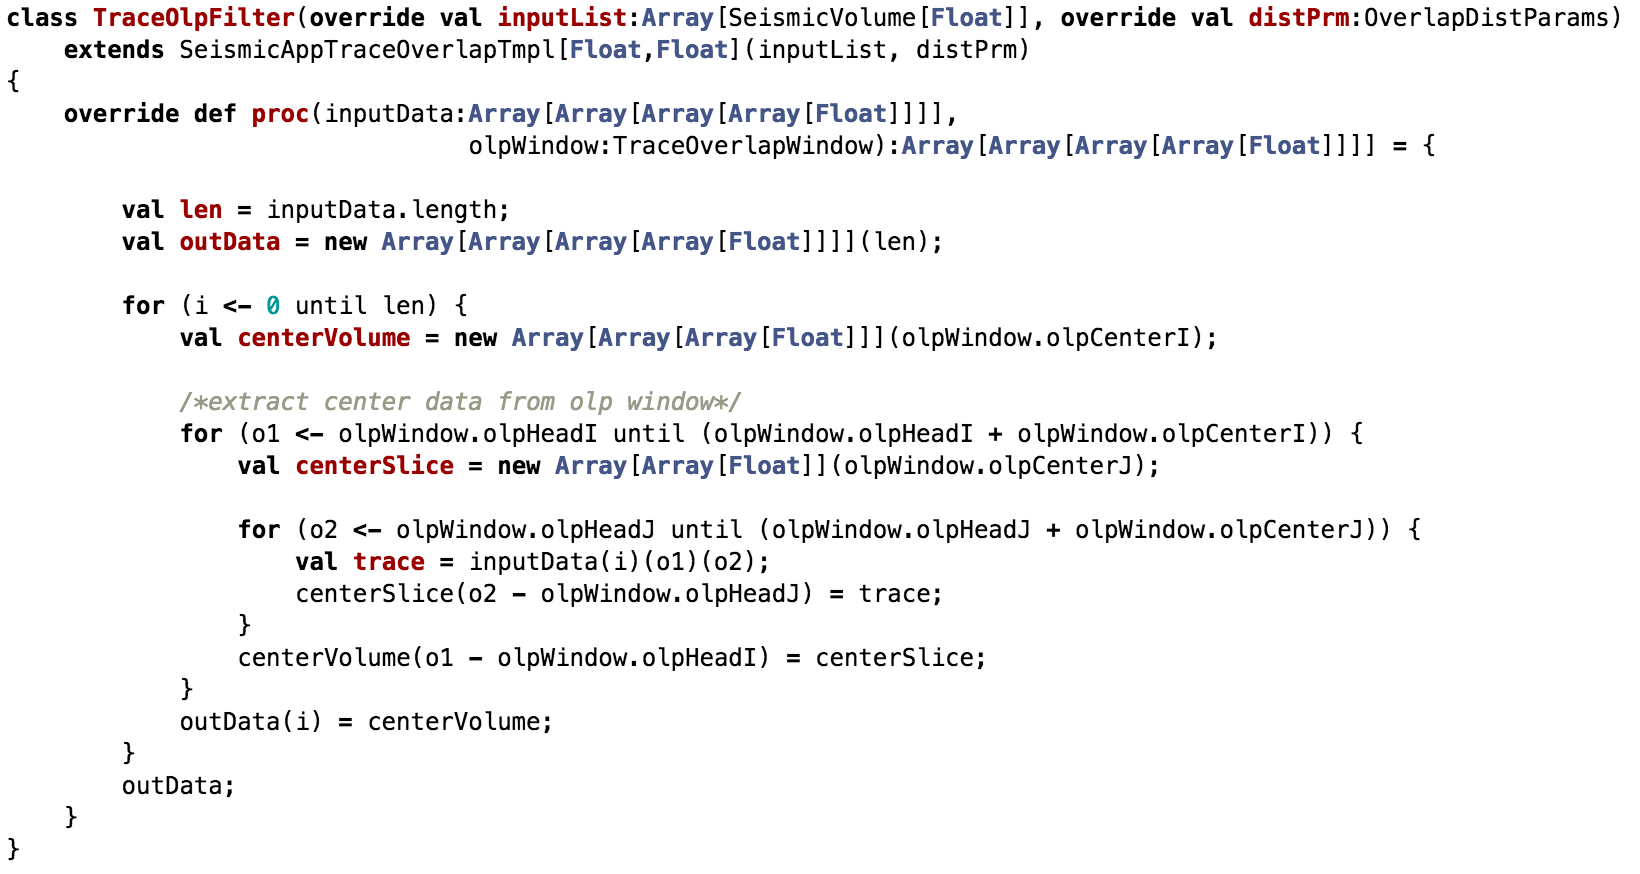
\includegraphics[scale=0.65]{figures/code_tmpl_subv.png}
\caption{Sample Code of Sub-volume Parallel Template}
\label{code_tmpl_subv}
\end{figure}

\begin{figure}[h]
\centering
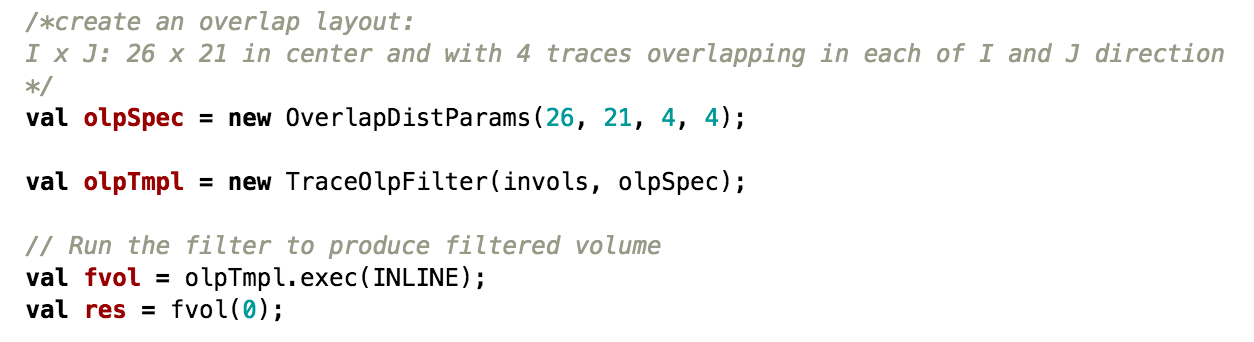
\includegraphics[scale=0.65]{figures/code_run_subv.png}
\caption{Sample Code of Executing Sub-volume Parallel Template}
\label{code_run_subv}
\end{figure}



%%%%%%%%%%%%%%%%%%%%%%%%%%%%%%%%%%%%%%%%%%%%%%%%%%%
%
%  New template code for TAMU Theses and Dissertations starting Fall 2012.  
%  For more info about this template or the 
%  TAMU LaTeX User's Group, see http://www.howdy.me/.
%
%  Author: Wendy Lynn Turner 
%	 Version 1.0 
%  Last updated 8/5/2012
%
%%%%%%%%%%%%%%%%%%%%%%%%%%%%%%%%%%%%%%%%%%%%%%%%%%%
%%%%%%%%%%%%%%%%%%%%%%%%%%%%%%%%%%%%%%%%%%%%%%%%%%%%%%%%%%%%%%%%%%%%%%
%%                           SECTION V
%%%%%%%%%%%%%%%%%%%%%%%%%%%%%%%%%%%%%%%%%%%%%%%%%%%%%%%%%%%%%%%%%%%%%


\chapter{\uppercase{Experiments, Results and Analysis}}

To verify and demonstrate the scalability that the user application could achieve through Seismic Data Analytics SDK, we conducted a series of experiments, including data transposing and 3D stencil calculation which resolves the overlapping-calculation problem. 

\section{3D Volume Transposing}

\subsection{Use Case}

This section presents the experiments of the 3D transposing problem mentioned in previous chapter. The dataset we used for transposing (from I  to J direction) experiment is a 300GB seismic 3D volumetric data, which is 31017 x 97223 x 31 in I x J x K direction with float data type. 
We design the experiment to verify the performance of transposing is scalable, and mainly affected by the data distribution configuration and the amount of available hardware resource(the number of cores).

\subsection{Statistics and Analysis}

\paragraph{Scalability to the Number of CPU Cores}

We conducted the transposing experiment on a cluster with 24 nodes, each node has 12 cores(24 cores in Hyper-threading) and 48GB available DRAM. The total CPU cores is 288(576 in Hyper-threading). Figure \ref{TestStat} shows the performance metrics of this experiment. The \emph{x} in \emph{Transpose[x]} stands for the aggregation parameter we applied on the dataset. As mentioned in previous chapter, the value of aggregation parameter \emph{x} specifies the number of planes in each data partition, thus to control the size of each data partition and the number of partitions. 

\begin{figure}[h]
\centering
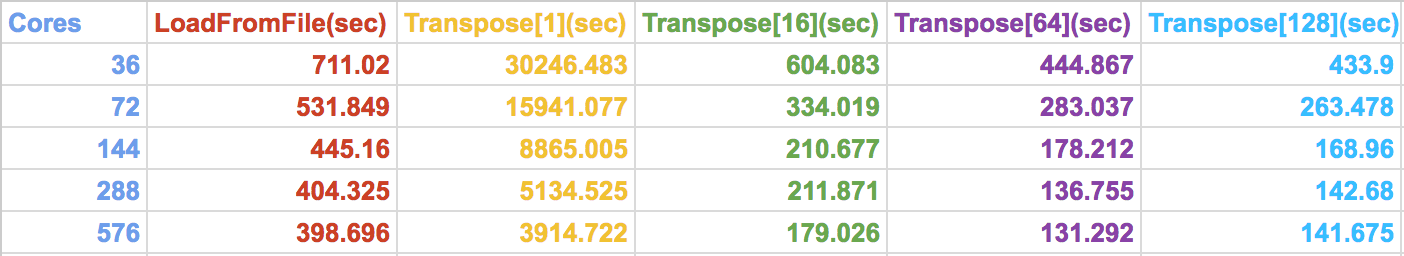
\includegraphics[scale=0.6]{figures/TestStat.png}\\
\caption{Transposing Experiment Statistics on Cluster with 288(576) cores.}\label{TestStat}
\end{figure}

From the statistics table, we generated two bar charts which show the time consuming for the transposing of aggregated and non-aggregated data. It clearly demonstrates that the performance scalability on dimension of the count of CPU cores is promised, as shown in Figure \ref{PerfTestCoresNoAgg} and  Figure \ref{PerfTestCoresAgg}. The performance difference between the transposing on aggregated and non-aggregated seismic volume data will be addressed in the following paragraphs.

\begin{figure}[ht]
\centering
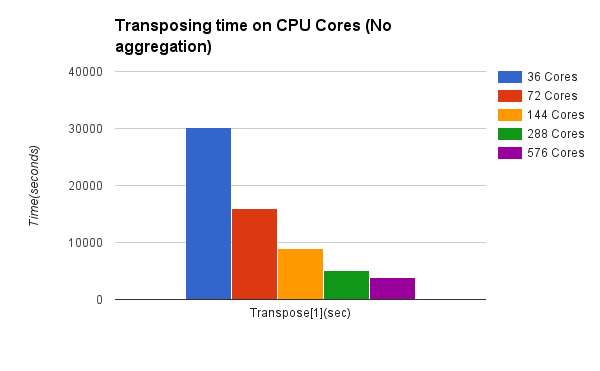
\includegraphics[scale=0.7]{figures/PerfTestCoresNoAgg.png}\\
\caption{Transposing Time on CPU Cores without Aggregation}\label{PerfTestCoresNoAgg}
\end{figure}

\begin{figure}[h]
\centering
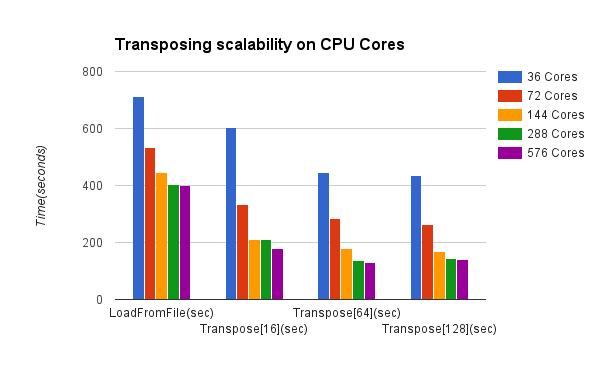
\includegraphics[scale=0.7]{figures/PerfTestCoresAgg.png}\\
\caption{Transposing Time on CPU Cores with Aggregation.}\label{PerfTestCoresAgg}
\end{figure}


\paragraph{Scalability to the Fashion of Data Distributions}

There is another important factor, the data distribution fashion, also affects the performance of transposing. As we mentioned in previous section, the transposing program will perform some shuffle operations on SeismicRDD. Shuffle operations \cite{SparkShuffle} is the mechanism for re-distributing data of a RDD so as to change the data partitions across the cluster. This process involves copying data across working nodes, which makes shuffle a complex and costly operation. To reduce the costs of shuffle operation, we aggregate the SeismicRDD data partitions to reduce the number of data splits, thus to reduce the amount of data exchanges during 3D transposing of the RDD data collection. Figure \ref{PerfTestAgg} shows the performance improvement when we increase the planes number (\emph{x} in \emph{Transpose[x]}) of each data distribution. 

\begin{figure}[h]
\centering
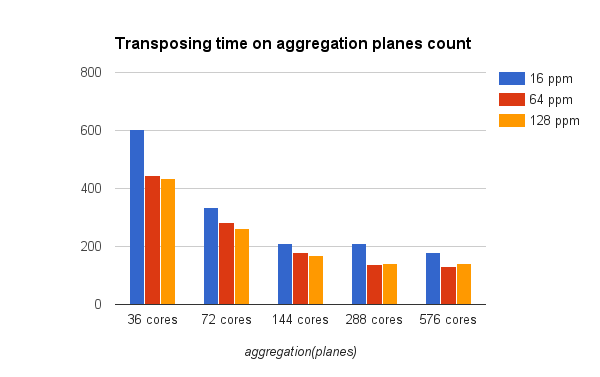
\includegraphics[scale=0.7]{figures/PerfTestAgg.png}\\
\caption{Transposing Time on Aggregated Planes(ppm: planesPerMap).}\label{PerfTestAgg}
\end{figure}

However, the curve of performance trends to flat when the decreasing aggregation number reaches to a certain threshold. That is caused by the performance trade-off of reducing the distribution partitions, which leads to a lower utilizing rate of cluster CPU cores than increasing the number partitions. Therefore, to achieve a reasonable performance for transposing process, developers need to considerate the trade-off between the distribution configurations and data shuffling carefully. 

Figure \ref{NMONCPU} and Figure \ref{NMONMEM} show the CPU utilization rate and memory usage of each node when the transposing experiment was running on the cluster. These system statistics diagrams were generated by a free software NMONVisualizer \cite{NMONVisualizer}, which is a Java GUI tool for analyzing NMON statistics files.
% from both AIX and Linux. 
%It also parses IOStat files, IBM verbose GC logs, Windows Perfmon and ESXTop CSV data and JSON data.

\begin{figure}[h]
\centering
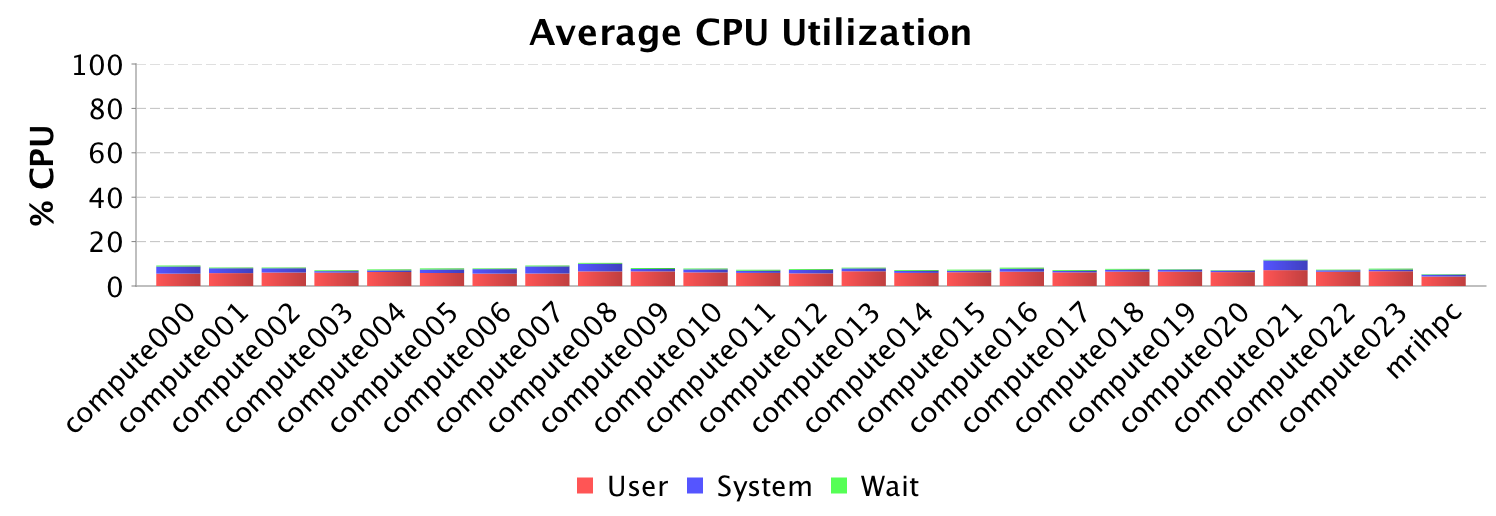
\includegraphics[scale=0.6]{figures/NMONCpu.png}\\
\caption{CPU utilization statistics from NMONVisualier.}\label{NMONCPU}
\end{figure}

\begin{figure}[h]
\centering
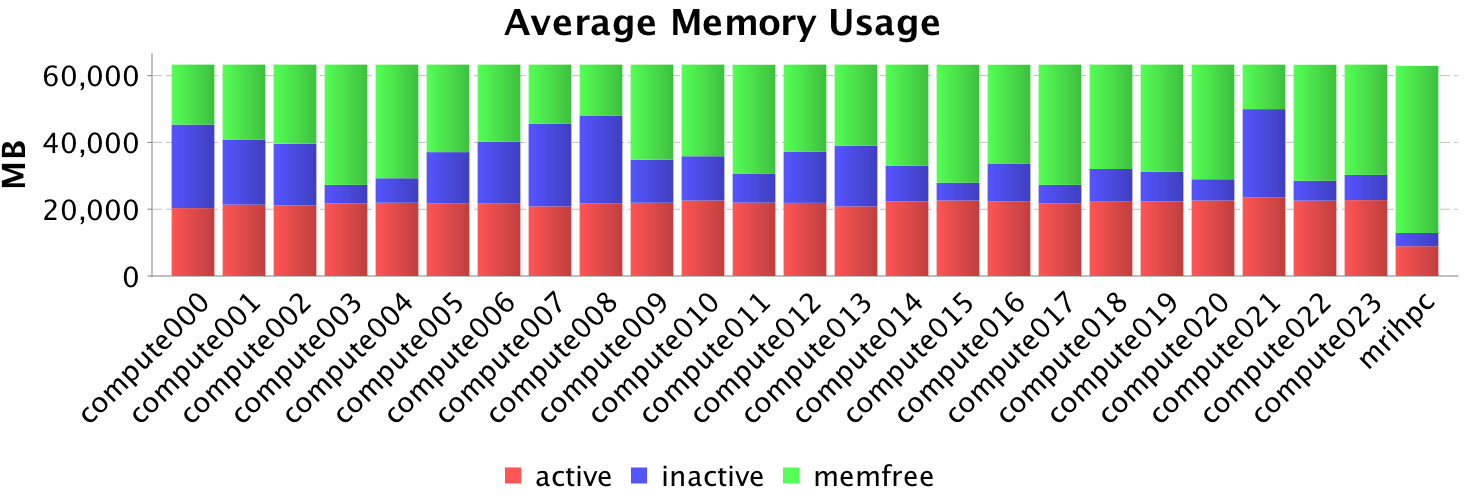
\includegraphics[scale=0.6]{figures/NMONMemory.png}\\
\caption{DRAM utilization statistics from NMONVisualier.}\label{NMONMEM}
\end{figure}

\paragraph{Cross-Verification on the Third-party Cloud Platform: XSEDE Cluster}

To further verify the scalability of transposing process, we also setup the same experiments on the third-party  commercial supercomputing cluster XSEDE \cite{XSEDE}. We requested 44 nodes from XSEDE cluster with 12 cores in each node. Figure \ref{XSEDETestStat} shows the statistics result of the experiments. As shown in Figure \ref{XSEDETest}, we conduct the experiments to test the performance of transposing the same seismic dataset from I to J direction with aggregation of 16 planes per partition. The result verified the scalability of this distributed solution.

\begin{figure}[h]
\centering
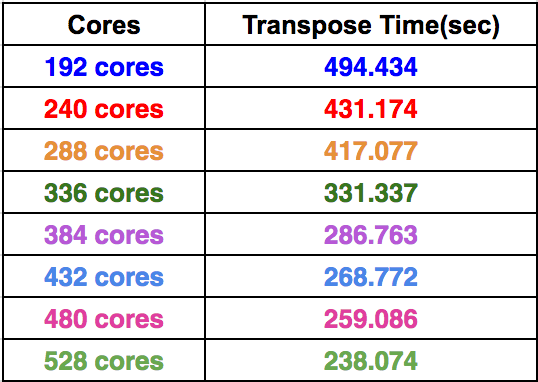
\includegraphics[scale=0.6]{figures/XSEDETestStat.png}\\
\caption{The Transposing Performance Statistics on XSEDE Cluster}\label{XSEDETestStat}
\end{figure}

\begin{figure}[h]
\centering
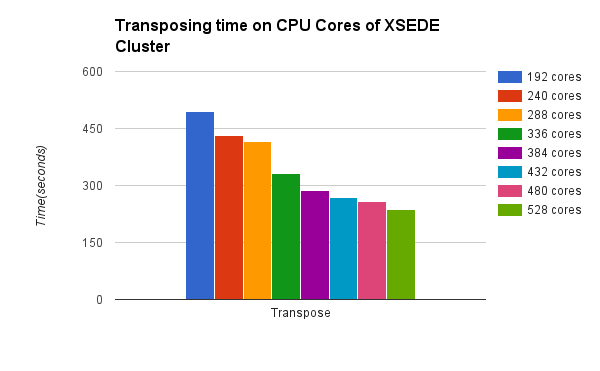
\includegraphics[width=0.8\textwidth]{figures/XSEDETest.png}\\
\caption{The Performance Scalability of Transposing on XSEDE Cluster }\label{XSEDETest}
\end{figure}


\section{3D Stencil Application}

\subsection{Use Case}

Stencil computations are most commonly used in the context of scientific and engineering applications, such as the signal and image processing, computer simulations etc.
Stencil computations itself represents an iterative kernel that updates array elements according to fixed pattens \cite{StencilWiki}. The optimization of stencil computation has been well studied in \cite{Han2011PADS},\cite{Nguyen2010Blocking} and \cite{Datta2008Stencil}. 
However, most of these optimizations focus on single node implementation with GPU or multi-core CPUs. In \cite{YanMasterThesis}, \cite{7363985} and \cite{7396203}, the authors provide the parallel implementation with Spark RDD, which gives a scalable solution for big data that can not host on a single node. 
%The approach simplifies the development efforts by underline complicate data distribution problem. 
In this experiment, we use the user-defined parallel template in Seismic Data Analytics SDK to resolve stencil computations. The experiments are designed and performed to test the performance and scalability.

\subsection{Statistics and Analysis}

The dataset we choose to conduct our experiment is called Penobscot dataset, which is actual seismic image data with 3D dimension size 600x481x1501. 
The cluster consists of 8 nodes, in which one is management node and other 7 nodes are computation nodes. Each node was equipped with Intel Xeon E5-2690 Sandy Bridge CPU (2.9 GHz, 16 Cores or 32 Cores with Hyper-threading support), 128GB DDR3 memory and are inter-connected with 1GB ethernet. 
JDK 1.8.0\_40, Hadoop 2.5.1 and Spark 1.6.1 are used for compiling and running applications. Wall clock is used to get the running time, and Nmon/Spark Web UI are used for performance analysis.

For the algorithm, we use a variant of Jacobi iteration, which uses a 3D subvolume with dimension size of 3x3x3 as input, and in the computation, each new output value at (i, j, k) is the average value of 26 surrounding samples plus itself. In the case of 3x3x3 subvolume, the overlap area is 1. 
For the sequential codes, we just split the big 3D data file into small partition and each partition includes several 2D planes (the overlap between partition is one 2D plane), and then use 3 nested loops to compute the average value. 
For the parallel codes using SDK, we use the overlapped template, which specify parameters both in I and J directions. 
Different configurations of cores and numbers of planes in each partition are set to check performance and scalability. 
The numbers of cores (28, 56, 112, 224) are used for each test case respectively to verify the scalability of parallel codes. 
Within each configuration of cores, we use different combinations of dimension size (1, 2, 4, 8) in I and J directions. For an instance, I(4) and J(2) mean that the dimension size of input subvolume 6x4, which comes from (4+2*1)x(2+2*1) in the case of overlap is 1, which is shown in Figure \ref{StencilData}.

\begin{figure}[h]
\centering
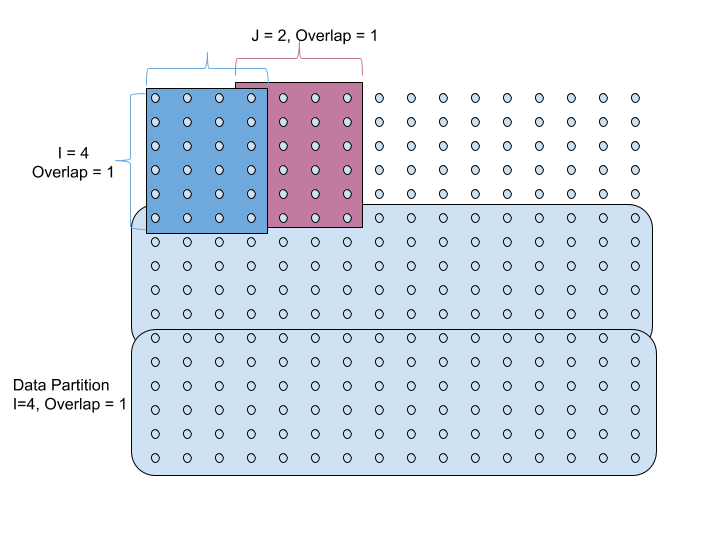
\includegraphics[scale=0.5]{figures/StencilData.png}\\
\caption{The Data Distributation and Input of Overlaop Template}
\label{StencilData}
\end{figure}

Figure \ref{Stencil28} and Figure \ref{Stencil224} show the speed up of parallel codes on Spark with 28 cores and 224 cores to the sequential codes respectively. 
From these two figures, the changes on number of \emph{J} have little impact on the performance, because it does not change the number of planes in each partition and the number of partitions. In the template implementation, two nested loops are used for feeding the input of each stencil kernel. However, the change on number of \emph{I} tells how the SDK distributes the data and the number of partitions, thus will determine how many tasks are need to finish that stage of in the job, and each task need to be assinged one thread or one core to undertake the computation.

In the case that size of \emph{I} is 1, it gets the best speed up in all test cases. It seems to be abnormal that the performance decreases from 1 plane of I to 2 planes of I. Increasing I will enlarge the size of each partition as shown in Figure \ref{StencilData}, however, the amount of computations keeps constant. In this stencil computation, we iterate several times to reach the balance. 

At the beginning of each loop, the data need to be repartitioned based on the overlap parameter, since the latest edge data need to be updated to each partition for next iteration. In the process of repartition, it needs to get planes at the left and right edge, sort them by key and zip with original latest results, which trigger data shuffle in Spark. The bigger the size of partitions is, the more time it takes to shuffle them. The 'Shuffle Read Blocked Time' increases drastically from 1 plane of I to 2 planes of I, which accounts for the performance decreasing. 
Figure \ref{StencilBest} shows the best speedup with different configurations of cores, in which the scalability is obvious while increasing the number of cores.

\begin{figure}[h]
\centering
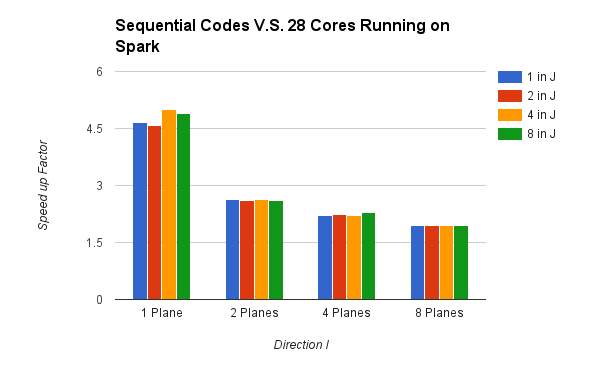
\includegraphics[scale=0.7]{figures/Stencil28.png}\\
\caption{The Speedup of Parallel Template Codes with 28 Cores to Sequential Codes}
\label{Stencil28}
\end{figure}

\begin{figure}[h]
\centering
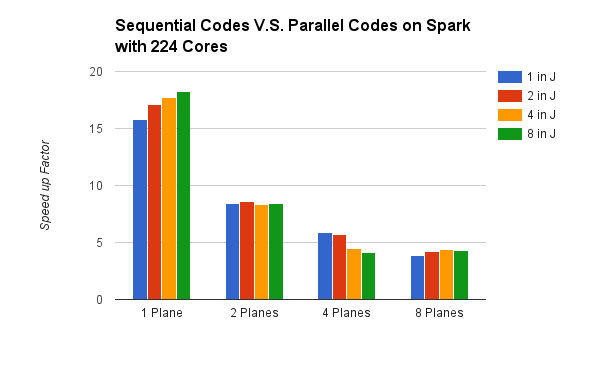
\includegraphics[scale=0.7]{figures/Stencil224.png}\\
\caption{The Speedup of Parallel Template Codes with 224 Cores to Sequential Codes}
\label{Stencil224}
\end{figure}

\begin{figure}[h]
\centering
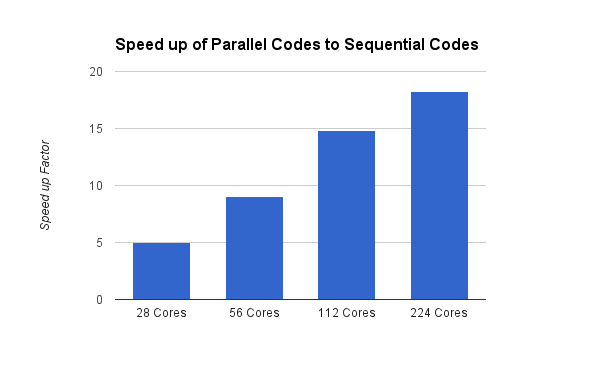
\includegraphics[scale=0.7]{figures/StencilBest.png}\\
\caption{The Best Speedup of Parallel Templates for Stencil Computation}
\label{StencilBest}
\end{figure}



%%%%%%%%%%%%%%%%%%%%%%%%%%%%%%%%%%%%%%%%%%%%%%%%%%
%
%  New template code for TAMU Theses and Dissertations starting Fall 2012.  
%  For more info about this template or the 
%  TAMU LaTeX User's Group, see http://www.howdy.me/.
%
%  Author: Wendy Lynn Turner 
%	 Version 1.0 
%  Last updated 8/5/2012
%
%%%%%%%%%%%%%%%%%%%%%%%%%%%%%%%%%%%%%%%%%%%%%%%%%%%
%%%%%%%%%%%%%%%%%%%%%%%%%%%%%%%%%%%%%%%%%%%%%%%%%%%%%%%%%%%%%%%%%%%%%%
%%                           SECTION IV
%%%%%%%%%%%%%%%%%%%%%%%%%%%%%%%%%%%%%%%%%%%%%%%%%%%%%%%%%%%%%%%%%%%%%

\chapter{\uppercase{Seismic Data Analytics Platform}}

In oil \& gas companies, the data analytics software is not only used by scientists and researchers, but also the employees who do not have the background of computer science. To allow those users to browse the seismic data and to generate analytics result, we developed some user-friendly utilities on top of Seismic Data Analytics SDK to simplify the way for deploying general purpose applications on Spark-Hadoop platform, which include a distributed data server for remote data access, the web interfaces for remote data visualization and user-defined workflow. With these tools, the users, not only the developers, are able to easily facilitate their works with this Seismic Data Analytics Platform in minimal efforts.


\section{Data Server and Remote Web Visualization}

In petroleum industry, an important application scenario is data visualization, which allows user to browse and analyze seismology features of seismic data in 3D spacing. With visualization tools, computer renders the seismic data to 3D graphic views and allows user to browse and manipulate the graph along any direction, which inspired the geophysicists and data scientists to develop various of useful models. However,traditional visualization tools in industry are only capable of handling small datasets, or render only few segments of the big datasets at a time. The performance of  big dataset visualization has long been the critical bottleneck of regular workflow of industry.

To resolve this problem, we developed a web-based remote data visualization service which is able to load and render the seismic data for 3D visualization in real-time. Figure \ref{visualization_framework} shows the framework of this service. 

\begin{figure}[h]
\centering
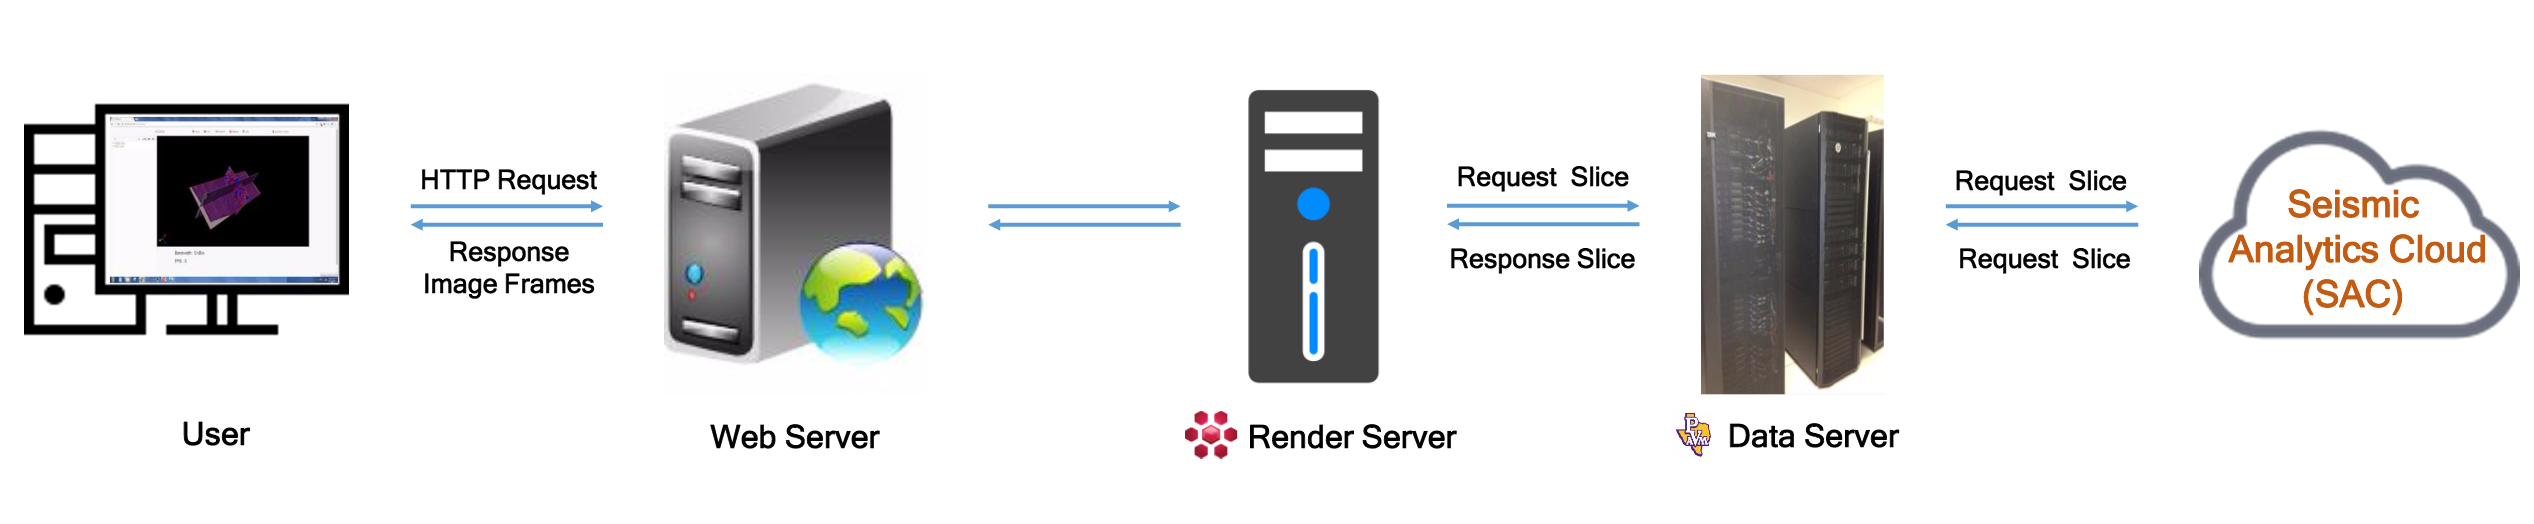
\includegraphics[scale=0.3]{figures/visualization_framework.png}
\caption{The Framework of Remote Web Visualization Service}
\label{visualization_framework}
\end{figure}

This solution is developed on top of Seismic Data Analytics SDK APIs and FEI Digital Rock Visualization Packages. We design and implement the DataServer service on top of Seismic Data Analytics SDK, which could load big seismic datasets from HDFS, transpose and store them to SeismicRDD in backends then feed the requested data in any direction to FEI visualization service in real-time. The FEI Digital Rock Visualization package is developed by FEI, the company which has been focus on featuring Digital Rock technology and solutions many years \cite{FEICompany}. 

Finally, the output rendered data view is presented through web interface and allows user to browse and manipulate in any direction. With this solution, user do not need to install complicated visualization tools and packages since the platform handles everything on server-side. More importantly, the performance of rendering big seismic data is improved and scalable after facilitated by Seismic Data Analytics SDK. Figure \ref{visualization} show s the web interface of this solution.

\begin{figure}[h]
\centering
\includegraphics[scale=0.3]{figures/visualization.png}
\caption{Visualization Web Interface}
\label{visualization}
\end{figure}


\section{Web-based Workflow Platform}

Another service we developed is a web-based workflow platform, which provides a friendly web interface to make cloud platform easy to use without programming, with which users could create workflow with drag and drop, could run the created workflow and check the results through visualization model. The Workflow Web Service is implemented on an open source project Clowdflows \cite{Clowdflows}, which provides a Django based framework to develop a customized widget and to manage widgets conveniently. As a free and open source web application framework written in Python, Django follows the Model, View and Controller (MVC) architectural pattern, so it is suitable for interact with both cloud service and web client.

The client side view of workflow is shown as Figure \ref{workflow}. Users could select widgets and specify seismic data files as input to construct and customize their workflows. Each widget in the workflow view is an independent application component which could be implemented on top of Seismic Data Analytics SDK. A widget acquires at least one port as input or output thus multiple widgets are able to be combined to a workflow by multiple pipelines which connect the ports of all widgets. Each pipeline in the workflow view indicates a data communication, which transports data between widgets and drives the execution of whole workflow. The workflow framework implemented by Python code includes Django views (GUI), Django models (widgets data management) and topological sorting algorithm (connections check).  The data files are stored in HDFS of the cloud platform and could be browsed and selected from the navigation trees on the editor page.

\begin{figure}[h]
\centering
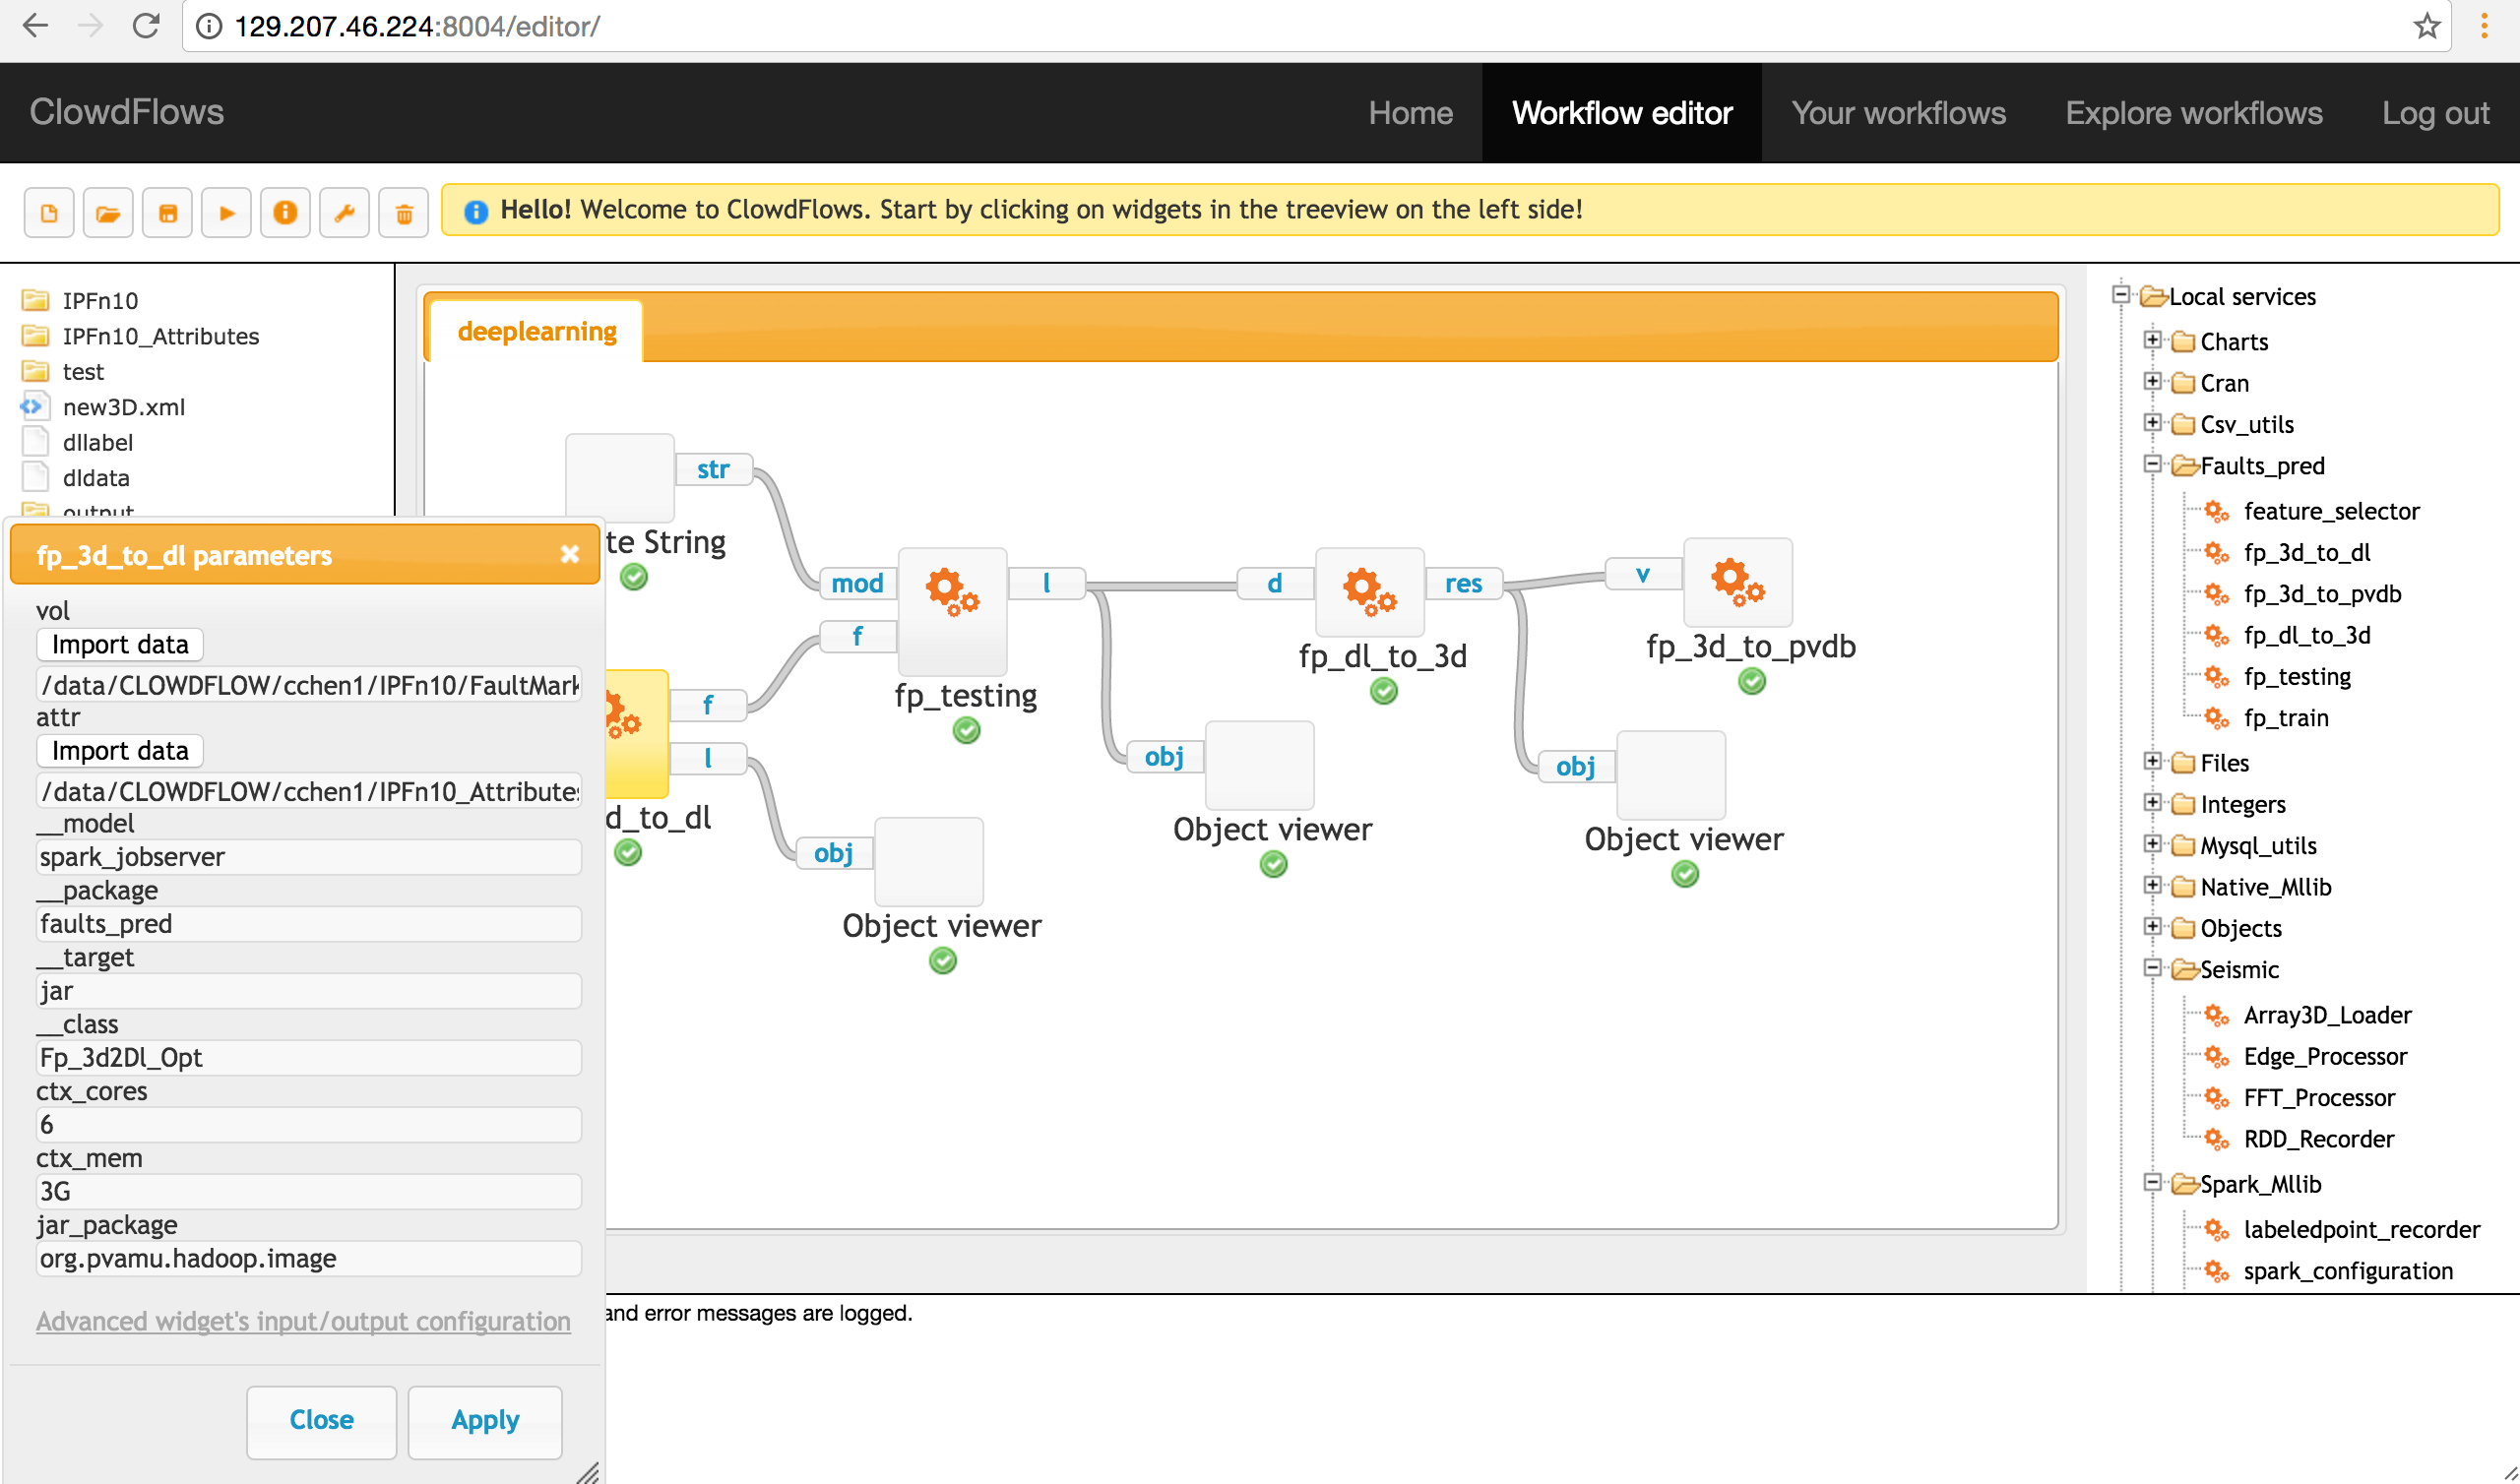
\includegraphics[scale=0.3]{figures/workflow.png}
\caption{Workflow Web Interface}
\label{workflow}
\end{figure}


%%%%%%%%%%%%%%%%%%%%%%%%%%%%%%%%%%%%%%%%%%%%%%%%%%%
%
%  New template code for TAMU Theses and Dissertations starting Fall 2012.  
%  For more info about this template or the 
%  TAMU LaTeX User's Group, see http://www.howdy.me/.
%
%  Author: Wendy Lynn Turner 
%	 Version 1.0 
%  Last updated 8/5/2012
%
%%%%%%%%%%%%%%%%%%%%%%%%%%%%%%%%%%%%%%%%%%%%%%%%%%%
%%%%%%%%%%%%%%%%%%%%%%%%%%%%%%%%%%%%%%%%%%%%%%%%%%%%%%%%%%%%%%%%%%%%%%
%%                           SECTION VI
%%%%%%%%%%%%%%%%%%%%%%%%%%%%%%%%%%%%%%%%%%%%%%%%%%%%%%%%%%%%%%%%%%%%%



\chapter{\uppercase{Conclusions and Future Work}}

The thesis presents a scalable and distributed Seismic Data Analytics toolkit that is implemented on top of Apache Hadoop and Spark big data platforms. It is an attempt to apply HPC optimizations to big seismic data analytics applications, and simplify the parallelism efforts. The experiments and related analysis given in this thesis also shows that this toolkit provides promised scalability, by which performance enhancement can be achieved by increasing cluster hardware resources or tuning distribution parameters without refactoring the application code.

In the future, advanced data distribution strategies such as tiling and bricking with 3D overlapping will be implemented for further improvement of the application performance. More application utilities and web service will be developed for data browsing and analytics purposes. We will put more efforts to provide a comprehensive Seismic Data Analytics Platform as a Service(PaaS) to facilitate the works of scientists. 


%%%%%%%%%%%%%%%%%%%%%%%%%%%%%%%%%%%%%%%%%%%%%%%%%%%%%%%
%\begin{figure}[H]
%\centering
%\includegraphics[scale=.50]{figures/Penguins.jpg}
%\caption{Another TAMU figure}
%\label{fig:tamu-fig4}
%\end{figure}
%%%%%%%%%%%%%%%%%%%%%%%%%%%%%%%%%%%%%%%%%%%%%%%%%%%%%%%




%fix spacing in bibliography, if any...
%%%%%%%%%%%%%%%%%%%%%%%%%%%%%%%%%%%%%%%%%%%%%%%%%%%%%%%%%%%%%
\let\oldbibitem\bibitem
\renewcommand{\bibitem}{\setlength{\itemsep}{0pt}\oldbibitem}
%%%%%%%%%%%%%%%%%%%%%%%%%%%%%%%%%%%%%%%%%%%%%%%%%%%%%%%%%%%%%%%
%%%%%%%%%%%%%%%%%%%%%%%%%%%%%%%%%%%%%%%%%%%%%%%%%%%
%
%  New template code for TAMU Theses and Dissertations starting Fall 2012.  
%  For more info about this template or the 
%  TAMU LaTeX User's Group, see http://www.howdy.me/.
%
%  Author: Wendy Lynn Turner 
%	 Version 1.0 
%  Last updated 8/5/2012
%
%%%%%%%%%%%%%%%%%%%%%%%%%%%%%%%%%%%%%%%%%%%%%%%%%%%


%%%%%%%%%%%%%%%%%%%%%%%%%%%%%%%%%%%%%%%%%%%%%%%%%%%%%%%%%%%%%%%%%%%%%%
%%                           REFERENCES 
%%%%%%%%%%%%%%%%%%%%%%%%%%%%%%%%%%%%%%%%%%%%%%%%%%%%%%%%%%%%%%%%%%%%%

\phantomsection
\addcontentsline{toc}{chapter}{REFERENCES}

\renewcommand{\bibname}{{\large\textbf\center REFERENCES}}

\bibliographystyle{plain}
\bibliography{references}

%%%%%%%%%%%%%%%%%%%%%%%%%%%%%%%%%%%%%%%%%%%%%%%%%%%%
%
%  New template code for TAMU Theses and Dissertations starting Fall 2012.  
%  For more info about this template or the 
%  TAMU LaTeX User's Group, see http://www.howdy.me/.
%
%  Author: Wendy Lynn Turner 
%	 Version 1.0 
%  Last updated 8/5/2012
%
%%%%%%%%%%%%%%%%%%%%%%%%%%%%%%%%%%%%%%%%%%%%%%%%%%%

\begin{appendices}
\titleformat{\chapter}{\centering\normalsize}{APPENDIX \thechapter}{0em}{\vskip .5\baselineskip\centering}
\renewcommand{\appendixname}{APPENDIX}

%%%%%%%%%%%%%%%%%%%%%%%%%%%%%%%%%%%%%%%%%%%%%%%%%%%
%
%  New template code for TAMU Theses and Dissertations starting Fall 2012.  
%  For more info about this template or the 
%  TAMU LaTeX User's Group, see http://www.howdy.me/.
%
%  Author: Wendy Lynn Turner 
%	 Version 1.0 
%  Last updated 8/5/2012
%
%%%%%%%%%%%%%%%%%%%%%%%%%%%%%%%%%%%%%%%%%%%%%%%%%%%

%%%%%%%%%%%%%%%%%%%%%%%%%%%%%%%%%%%%%%%%%%%%%%%%%%%%%%%%%%%%%%%%%%%%%%
%%                           APPENDIX A 
%%%%%%%%%%%%%%%%%%%%%%%%%%%%%%%%%%%%%%%%%%%%%%%%%%%%%%%%%%%%%%%%%%%%%

\phantomsection

\chapter{\uppercase{First Appendix}}

Text for the Appendix follows.

\begin{figure}[H]
\centering
\includegraphics[scale=.50]{figures/Penguins.jpg}
\caption{TAMU figure}
\label{fig:tamu-fig5}
\end{figure}

%%%%%%%%%%%%%%%%%%%%%%%%%%%%%%%%%%%%%%%%%%%%%%%%%%%
%
%  New template code for TAMU Theses and Dissertations starting Fall 2012.  
%  For more info about this template or the 
%  TAMU LaTeX User's Group, see http://www.howdy.me/.
%
%  Author: Wendy Lynn Turner 
%	 Version 1.0 
%  Last updated 8/5/2012
%
%%%%%%%%%%%%%%%%%%%%%%%%%%%%%%%%%%%%%%%%%%%%%%%%%%%

%%%%%%%%%%%%%%%%%%%%%%%%%%%%%%%%%%%%%%%%%%%%%%%%%%%%%%%%%%%%%%%%%%%%%%
%%                           APPENDIX B
%%%%%%%%%%%%%%%%%%%%%%%%%%%%%%%%%%%%%%%%%%%%%%%%%%%%%%%%%%%%%%%%%%%%%

\chapter{\uppercase {Second Appendix with a longer title - much longer in fact}}

Text for the Appendix follows.

\begin{figure}[H]
\centering
\includegraphics[scale=.50]{figures/Penguins.jpg}
\caption{TAMU figure}
\label{fig:tamu-fig6}
\end{figure}

\section{Appendix Section}


\pagebreak{}

\end{appendices}


\chapter*{CURRICULUM VITA}
\addcontentsline{toc}{chapter}{VITA}  % Needs to be set to part, so the TOC doesnt add 'CHAPTER ' prefix in the TOC.

% Comment the following lines to use the default Computer Modern font
% instead of the Palatino font provided by the mathpazo package.
% Remove the 'osf' bit if you don't like the old style figures.

% Set your name here
\def\name{Chao Chen}

% Don't indent paragraphs.
\setlength\parindent{0em}

% Make lists without bullets
\renewenvironment{itemize}{
  \begin{list}{}{
    \setlength{\leftmargin}{1.5em}
  }
}{
  \end{list}
}

% Place name at left
\section*{\large \bf \name}
\begin{singlespace}

\begin{minipage}{0.45\linewidth}
  Prairie View A\&M University \\
  Department of Computer Science \\
  P.O. Box 519, Prairie View, 77446
\end{minipage}
\begin{minipage}{0.45\linewidth}
  \begin{tabular}{ll}
    Phone: & (832) 910-4615 \\
    Email: & \url{cchen.rough@gmail.com} \\
  \end{tabular}
\end{minipage}


\section*{\large \bf Education}

\begin{itemize}
  \item M.S. Computer Science, Prairie View A\&M University, 2016.

  \item B.A. Electronic Information Engineering, Southwest University of Science and Technology, 2005.

\end{itemize}

\section*{\large \bf Employment}

\begin{itemize}
\item Prairie View A\&M University, Research Assitant, 2015--2016.
\item Sunmedia Technology, Software Engineer, 2006--2014.
\end{itemize}


\section*{\large \bf Professional Skills}
\begin{itemize}
\item Solid background of computer science and software engineering, as well as strong learning and communication ability.
\item Proficient at Linux, Android and Embedded OS development, strong products development experiences including digital camera, digital photo frame and tablet.
\item Familiar with big data and cloud computing platform (Hadoop, Spark).
\end{itemize}



\section*{\large \bf Publications \& Achievements}

%\subsection*{Journal Articles}

\begin{itemize}

\item A Scalable and Productive Workflow-based Cloud Platform for Big Data Analytics, {\it 2016 IEEE International Conference on Big Data Analysis}, (ICBDA 2016) Hangzhou, China, March 12-14, 2016

\item A Productive Cloud Computing Platform Research for Big Data Analytics, {\it In Proc. of IEEE CloudCom 2015}, Nov 30-Dec 3, Vancouver, Canada

\end{itemize}

\end{singlespace}

% Footer
%\begin{center}
%  \begin{footnotesize}
%    Last updated: \today \\
%  \end{footnotesize}
%\end{center}





\end{document}
